%definira klasu dokumenta 
\documentclass[12pt]{report} 

%prostor izmedu naredbi \documentclass i \begin{document} se zove uvod. U njemu se nalaze naredbe koje se odnose na cijeli dokument

%osnovni LaTex ne može riješiti sve probleme, pa se koriste različiti paketi koji olakšavaju izradu željenog dokumenta
\usepackage[croatian]{babel}  
\usepackage{amssymb}
\usepackage{amsmath}
\usepackage{txfonts}
\usepackage{mathdots}
\usepackage{titlesec}
\usepackage{array}
\usepackage{lastpage}
\usepackage{etoolbox}
\usepackage{tabularray}
\usepackage{color, colortbl}
\usepackage{adjustbox}
\usepackage{geometry}
\usepackage[classicReIm]{kpfonts}
\usepackage{hyperref}
\usepackage{fancyhdr}

\usepackage{float}
\usepackage{setspace}
\restylefloat{table}


\patchcmd{\chapter}{\thispagestyle{plain}}{\thispagestyle{fancy}}{}{} %redefiniranje stila stranice u paketu fancyhdr

%oblik naslova poglavlja
\titleformat{\chapter}{\normalfont\huge\bfseries}{\thechapter.}{20pt}{\Huge}
\titlespacing{\chapter}{0pt}{0pt}{40pt}


\linespread{1.3} %razmak između redaka

\geometry{a4paper, left=1in, top=1in,}  %oblik stranice

\hypersetup{ colorlinks, citecolor=black, filecolor=black, linkcolor=black,	urlcolor=black }   %izgled poveznice


%prored smanjen između redaka u nabrajanjima i popisima
\newenvironment{packed_enum}{
	\begin{enumerate}
		\setlength{\itemsep}{0pt}
		\setlength{\parskip}{0pt}
		\setlength{\parsep}{0pt}
	}{\end{enumerate}}

\newenvironment{packed_item}{
	\begin{itemize}
		\setlength{\itemsep}{0pt}
		\setlength{\parskip}{0pt}
		\setlength{\parsep}{0pt}
	}{\end{itemize}}




%boja za privatni i udaljeni kljuc u tablicama
\definecolor{LightBlue}{rgb}{0.9,0.9,1}
\definecolor{LightGreen}{rgb}{0.9,1,0.9}

%Promjena teksta za dugačke tablice
\DefTblrTemplate{contfoot-text}{normal}{Nastavljeno na idućoj stranici}
\SetTblrTemplate{contfoot-text}{normal}
\DefTblrTemplate{conthead-text}{normal}{(Nastavljeno)}
\SetTblrTemplate{conthead-text}{normal}
\DefTblrTemplate{middlehead,lasthead}{normal}{Nastavljeno od prethodne stranice}
\SetTblrTemplate{middlehead,lasthead}{normal}

%podesavanje zaglavlja i podnožja

\pagestyle{fancy}
\lhead{Programsko inženjerstvo}
\rhead{Wild Track}
\lfoot{Aristos}
\cfoot{stranica \thepage/\pageref{LastPage}}
\rfoot{\today}
\renewcommand{\headrulewidth}{0.2pt}
\renewcommand{\footrulewidth}{0.2pt}


\begin{document} 
	
	
	
	\begin{titlepage}
		\begin{center}
			\vspace*{\stretch{1.0}} %u kombinaciji s ostalim \vspace naredbama definira razmak između redaka teksta
			\LARGE Programsko inženjerstvo\\
			\large Ak. god. 2023./2024.\\
			
			\vspace*{\stretch{3.0}}
			
			\huge Wild Track\\
			\Large Dokumentacija, Rev. 2.\\
			
			\vspace*{\stretch{12.0}}
			\normalsize
			Grupa: \textit{Aristos}\\
			Voditelj: \textit{Josipa Udovičić}\\
			
			
			\vspace*{\stretch{1.0}}
			Datum predaje: \textit{19. siječnja 2024.}\\
	
			\vspace*{\stretch{4.0}}
			
			Nastavnik: \textit{Hrvoje Nuić}\\
		
		\end{center}

	
	\end{titlepage}

	
	\tableofcontents


	\chapter{Dnevnik promjena dokumentacije}
						
		
		\begin{longtblr}[
				label=none
			]{
				width = \textwidth, 
				colspec={|X[2]|X[13]|X[3]|X[3]|}, 
				rowhead = 1
			}
			\hline
			\textbf{Rev.}	& \textbf{Opis promjene/dodatka} & \textbf{Autori} & \textbf{Datum}\\[3pt] \hline
			0.1 & Napravljen predložak.	& Franjo Vuković & 04.11.2023. 		\\[3pt] \hline 
			0.2	& Dodani opis projektnog zadatka i \newline funkcionalni zahtjevi. & Josipa Udovičić & 04.11.2023. 	\\[3pt] \hline 
			0.2.1 & Promijenjen opis i funkcionalni zahtjevi. & Josipa Udovičić & 05.11.2023.  \\[3pt] \hline 
			0.3 & Dodan dio opisa obrazaca uporabe. & Stela Troskot & 05.11.2023. \\[3pt] \hline 
			0.3.1 & Dodani svi opisi obrazaca uporabe. & Stela Troskot, Domagoj Jurič & 05.11.2023.  \\[3pt] \hline 
			0.4 & Dodani dijagrami obrazaca uporabe. & Franjo Vuković, Marko Kukolj, Marko Pongrac & 05.11.2023. \\[3pt] \hline 
			0.5 & Dodani sekvencijski dijagrami. & Franjo Vuković, Marko Kukolj, Marko Pongrac & 08.11.2023.  \\[3pt] \hline 
			0.5.1 & Promijenjeni dijagrami obrazaca uporabe. & Stela Troskot, Domagoj Jurič & 09.11.2023. \\[3pt] \hline  
			0.5.2 & Dodan opis sekvencijskih dijagrama. & Marko Kukolj & 09.11.2023.  \\[3pt] \hline 
			0.5.3 & Dodani ostali zahtjevi. & Josipa Udovičić & 09.11.2023.   \\[3pt] \hline
			0.6 & Dodan opis arhitekture. & Josipa Udovičić & 09.11.2023.  \\[3pt] \hline 
			0.7 & Napravljena baza podataka. & Franjo Vuković, Marko Pongrac & 09.11.2023.  \\[3pt] \hline 
			0.7.1 & Napravljen dijagram baze podataka. & Franjo Vuković, Marko Pongrac & 09.11.2023.  \\[3pt] \hline 
			0.7.2 & Napisan opis baze podataka. & Gregor Mihaljević & 13.11.2023. \\[3pt] \hline 
			0.8 & Dodan dio dijagrama razreda. & Franjo Vuković, Marko Pongrac, Marko Kukolj & 15.11.2023. \\[3pt] \hline 
			0.8.1 & Dodani svi dijagrami razreda. & Franjo Vuković, Marko Pongrac, Marko Kukolj & 16.11.2023. \\[3pt] \hline 
			0.9 & Opisi razreda i dodatak & Josipa Udovičić & 16.11.2023. \\[3pt] \hline
			1.0 & Korigiranje teksta i provjera dokumentacije & Josipa Udovičić & 17.11.2023. \\[3pt] \hline
			1.1 & Implementacija. & Josipa Udovičić, Franjo Vuković, Marko Pongrac, Marko Kukolj, Domagoj Jurič & 16.01.2024. \\[3pt] \hline
			1.2 & Ispravljeni dijelovi prve predaje. & Stela Troskot, Josipa Udovičić, Franjo Vuković, Marko Kukolj & 17.01.2024. \\[3pt] \hline
			1.3 & Dodan dijagram stanja i dijagram aktivnosti. & Stela Troskot & 07.01.2024. \\[3pt] \hline
			1.4 & Dodan dijagram komponenti. & Stela Troskot & 09.01.2024. \\[3pt] \hline
			1.5 & Dodan dijagram razmještaja. & Stela Troskot & 11.01.2024. \\[3pt] \hline
			1.6 & Dodan opis tehnologija i alata. & Stela Troskot & 13.01.2024. \\[3pt] \hline
			1.7 & Ispitivanje programskih rješenja. & Marko Pongrac & 19.01.2024. \\[3pt] \hline
			1.8 & Dodane upute za puštanje u pogon. & Stela Troskot & 19.01.2024. \\[3pt] \hline
			1.9 & Dodan zaključak. & Stela Troskot & 19.01.2024. \\[3pt] \hline
			2.0 & Konačna verzija dokumentacije. & Stela Troskot & 19.01.2024. \\[3pt] \hline


		\end{longtblr}
	
	\chapter{Opis projektnog zadatka}
		
	Cilj ovog projekta je razviti programsku podršku za web aplikaciju "Wild Track".
	Ta aplikacija olakšava korisniku pronalazak i praćenje divljih životinja.
	Prilikom otvaranja aplikacije prikazuje se stranica za prijavu te opcija za registraciju.	
	
	Neregistriranom korisniku omogućeno mu je prijavljivanje u sustav s postojećim računom (potrebno je upisati korisničko ime i lozinku) ili kreiranje novog računa. 
	Za kreiranje novog računa potrebni su sljedeći podaci: 
	\begin{packed_item}
		\item uloga za koju se prijavljuje - može biti istraživač, voditelj postaje ili tragač na terenu
		\item korisničko ime 
		\item fotografija
		\item lozinka
		\item ime
		\item prezime
		\item email adresa
	\end{packed_item}

	Registracijom u sustav korisniku se dodjeljuju prava istraživača, voditelja postaje, tragača na terenu ili administratora.
	Registrirani korisnik može, uz opcije koje ima njegova željena uloga, još i pregledati te mijenjati osobne podatke.

	Registracija je završena kad korisnik preko svoje email adrese potvrdi, osim ako je korisnik izabrao biti istraživač ili voditelj postaje. 
	U tom slučaju, administrator mora potvrditi njihovu ulogu. 
	Administrator sustava ima najveće ovlasti. 
	On ima ovlasti da vidi popis svih registriranih korisnika i njihovih osobnih podataka, odnosno pristup bazi s popisom registriranih korisnika, te može mijenjati njihova dodijeljena prava i osobne podatke.
	
	Voditelj postaje može izabrati koji će tragači biti dio njegove postaje i bira na koji način oni mogu izvoditi pretraživanje životinja. 
	Postaje su određena mjesta na karti koja admin bira kada potvrđuje voditelja, to na primjer može biti postaja Biokovo ili postaja Lonjsko polje.
	Voditelj može pregledati aktivne i neaktivne akcije. Na aktivne akcije može dodati tragače koji su dio njegove postaje. Tragači se na akciju mogu dodavati i nakon pregleda zahtjeva od istraživača.
	Načine transporta za koji su njegovi tragači osposobljeni voditelj može promijeniti u svakom trenutku.

	Ako se korisnik prijavi kao tragač, njemu se na karti mogu prikazati zadaci koje mora obaviti, trenutna pozicija ostalih tragača koji su aktivni na istoj akciji, te trenutna pozicija životinja koje prati.
	Praćene životinje imaju na sebi gps uređaj koji aplikaciji odašilje njihovu poziciju i tako korisnik može cijelo vrijeme znati njihovu točnu lokaciju. 
	Tragač tijekom svoje akcije može ostavljati komentare o životinji koju je pratio te također može ostaviti komentar ostalim tragačima i istraživačima, to jest drugim sudionicima u akciji.
	Također, cijeli put koji tragači prođu se bilježi, odnosno označavaju se staze kojima su putovali i način kojim su se kretali. To će biti potrebno istraživačima koji vizualiziraju njihovo kretanje u obliku toplinskih karata 
	te potom to koriste za analiziranje kretanja životinja i njihovih omiljenih staništa. Tragač može i pregledati podatke o pojedinačnim životinjama(latinski naziv, sliku, opis i komentare). 
	Načini kojima se tragači kreću mogu biti različiti, kao na primjer:
	\begin{packed_item}
		\item pješke
		\item dronom
		\item automobilom
		\item cross motorom
		\item brodom
		\item helikopterom
	\end{packed_item}

	Ovisno o tome kojom je tragač metodom osposobljen za obavljanje zadataka, svaka metoda je drugačije prikazana na karti.
	Ako je tragač odabran da ide pješke njegova će karta biti detaljnija i prikazana na manjem prostoru nego karta tragača koji putuje helikopterom. 
	Svaki tragač koristi samo jednu vozilo i tijekom te akcije se njegov tip prijevoza ne mijenja.

	Ako je korisnik odlučio biti istraživač, on može stvoriti nove akcije pretraživanja i praćenja životinja s detaljima o određenim vrstama, jedinkama ili staništima za proučavanje.
	Svaki istraživač je zadužen za jednu akciju.
	Ako je istraživaču potreban tragač za pomoć pri istraživanju, istraživač može poslati voditelju postaje zahtjev za tragačima s opisom o potrebnim kvalifikacijama.
	Voditelj će na taj zahtjev odabrati tragače koji odgovaraju opisu i postaviti ih da sudjeluju u toj akciji.
	Tragač će biti gotov s akcijom kad završi sve potrebne zadatke.
	Istraživač, kad dobije određene tragače, zadaje preko karte zadatke pojedinačno svakom tragaču.
	Zadaci mogu biti različiti, kao na primjer prolazak određenom rutom i dolazak do određene lokacije te postavljanje kamere ili uređaja za praćenje.
	Prilikom postavljanja zadatka, istraživač može i ostaviti neke dodatne komentare tragačima.
	Informacije o poziciji životinje, tragaču i postaji se istraživaču prikazuju preko interaktivne karte.
	Istraživač može birati da se tijekom izrade karte koriste i neke određene informacije. Na primjer:
	\begin{packed_item}
		\item povijesne pozicije praćenih životinja
		\item filtriranje životinja po vrsti ili pojedinačno po jedinki
		\item trenutne pozicije praćenih životinja
		\item povijesne pozicije svih tragača na nekoj akciji
		\item filtriranje po tipu prijevoza ili pojedinačno po tragaču
		\item trenutne pozicije tragača koji su aktivni na akciji
	\end{packed_item}


	

	Ovaj projekt može biti korisan svima koji bi htjeli više naučiti o divljim životinjama, ali isto tako i ljudima koji se bave proučavanjem životinja može olakšati posao.
	Svaka osoba koja želi može se ulogirati i postati tragač, u svrhu zabave, dodatnog znanja... A time, dok ljudi to rade iz zabave, odnosno svojevoljno, osobe koji su istraživači 
	mogu koristiti njihove informacije i time im se smanjuje dio posla.

	Slične aplikacije poput aplikacije "Wild Track" na području Hrvatske ne postoje. Neke aplikacije koje se bave divljim životinjama su: "eWildLife" i "Divlje životinje".

	"eWildLife" je aplikacija razvijena u realnom vremenu, ljudi prate i izvještavaju o ubijanju divljih životinja, 
	sukobe čovjek-životinja i viđenja divljih životinja, također mogu i spasiti delfine. 

	"Divlje životinje" (Slika \ref{fig:divlje_zivotinje}) je Android aplikacija koja omogućuje istraživanje svijeta životinja. 
	Aplikacija nudi opsežan katalog divljih životinja, uključujući šumske životinje, životinje iz zooloških vrtova, cirkuske životinje, afričke životinje, šumske životinje itd. 
	Aplikacija pruža detaljan opis svake životinje, uključujući njezinu vrstu, veličinu, kao i podatke o ponašanju i navikama. 
	Također možete pristupiti raznim slikama koje će vam pomoći da bolje razumijete životinje. 

	\begin{figure}[H]
		\includegraphics[scale=0.4]{slike/divlje_zivotinje.png} %veličina slike u odnosu na originalnu datoteku i pozicija slike
		\centering
		\caption{Aplikacija Divlje Životinje}
		\label{fig:divlje_zivotinje}
	\end{figure}

	No, slična aplikacija "Wild Track" aplikaciji izvan Hrvatske postoji. Zove se "Animal Tracker" (Slika \ref{fig:animal_tracker}). 
	S pomoću "Animal Tracker" aplikacije moguće je pratiti kretanje divljih životinja diljem svijeta koje se prate u gotovo stvarnom vremenu.
	Kretanja se prikupljaju GPS oznakama koje životinje nose i pohranjuju se u Movebank (internetska infrastruktura koju koriste istraživači za upravljanje, dijeljenje, analizu i arhiviranje podataka o kretanju životinja).


	\begin{figure}[H]
		\includegraphics[scale=0.4]{slike/animal_tracker.png} %veličina slike u odnosu na originalnu datoteku i pozicija slike
		\centering
		\caption{Aplikacija Animal Tracker}
		\label{fig:animal_tracker}
	\end{figure}
	

	Poboljšanja na aplikacijama se uvijek mogu napraviti, pa tako može i na ovoj. Na primjer, moguće je pratiti otkucaje srca životinja, disanje\dots 
	Time je moguće određivati zdravlje životinje, kretnje životinje, da li životinja spava ili je budna\dots
	Tu smo dobili nove komponente aplikacije koje se mogu nazvati trenutne aktivnosti životinje i zdravlje životinje te tu tragači i istraživači imaju još više informacija o životinjama, a ne samo one općenite.
	Isto tako možemo dodati tragačima opciju da slikaju i snimaju životinje te im dati mogućnost da slike i videe objavljuju na aplikaciju. Time je opet doživljaj određene životinje bolji, a ne općenit.
	Aplikaciju bi svakako mogli poboljšati i tako da napravimo vizualno privlačniji i moderniji UI.

	
	\chapter{Specifikacija programske potpore}
		
	\section{Funkcionalni zahtjevi}
			
			\noindent \textbf{Dionici:}
			
			\begin{packed_enum}
				\item Tragač na terenu
				\item Istraživač				
				\item Voditelj postaje
				\item Administrator
				\item Razvojni tim
				
			\end{packed_enum}
			
			\noindent \textbf{Aktori i njihovi funkcionalni zahtjevi:}
			
			
			\begin{packed_enum}
				\item  \underbar{Neregistrirani korisnik  (inicijator) može:}
				
				\begin{packed_enum}
					\item se registrirati u sustav
					 \begin{packed_enum}
						\item  dati svoje podatke: korisničko ime, fotografija, lozinka, ime, prezime i email adresa
						\item  odabrati svoju ulogu(tragač, istraživač ili voditelj postaje)
						\item potvrditi registraciju na svojoj email adresi 
					\end{packed_enum}
				\end{packed_enum}
			
				\item  \underbar{Korisnik (inicijator) može:}
				
				\begin{packed_enum}
					\item se prijaviti u sustav
					\item upravljati svojim podatcima
					 \begin{packed_enum}
						\item  pregled osobnih podataka
						\item promjena osobnih podataka
						\item brisanje korisničkog računa
					\end{packed_enum}
				\end{packed_enum}

				\item  \underbar{Tragač (inicijator) na terenu  može:}
				
				\begin{packed_enum}
					
					\item vidjeti zadatke tijekom akcije
					 \begin{packed_enum}
						\item označiti da je zadatak riješen
					\end{packed_enum}
					\item završiti akciju
					\item vidjeti gdje se nalaze ostali tragači na akciji 
					\item vidjeti koje su dostupne akcije 
					 \begin{packed_enum}
						\item prihvatiti akciju
						\item odbiti akciju
					\end{packed_enum} 
					\item vidjeti pozicije praćenih životinja
					\item odabrati vozilo kojim će ići u istraživanje
					\item vidjeti informacije o životinjama
					 \begin{packed_enum}
						\item dodati komentar
						\item izbrisati komentar
					\end{packed_enum}

					
				\end{packed_enum}

				\item  \underbar{Istraživač (inicijator) može:}
				
				\begin{packed_enum}

					\item vidjeti informacije o životinjama
					 \begin{packed_enum}
						\item dodati komentar
						\item izbrisati komentar
					\end{packed_enum}
					\item vidjeti kartu 
					 \begin{packed_enum}
						\item izraditi kartu: na temelju životinja ili tragača
					\end{packed_enum}
					\item stvoriti novu akciju
					 \begin{packed_enum}
						\item dodati nove zadatke
					\end{packed_enum}
					\item poslati voditelju postaje zahtjev za tragačima
					 \begin{packed_enum}
						\item dodati tražene kvalifikacije tragača
					\end{packed_enum}
					\item zadati zadatke tragačima
					 \begin{packed_enum}
						\item upravljati zadacima
						 \begin{packed_enum}
							\item dodavati zadatke
							\item uređivati zadatke
							\item brisati zadatke
						\end{packed_enum}
						\item dodati komentare na zadatke
					\end{packed_enum}
					\item pregledati informacije


				\end{packed_enum}

				\item  \underbar{Voditelj postaje (inicijator) može:}
				
				\begin{packed_enum}
					\item pregledati sve tragače
					\item dodati tragača na akciju
					\item dodijeliti postaju tragaču
				\end{packed_enum}

				\item  \underbar{Administrator (inicijator) može:}
				
				\begin{packed_enum}
					\item vidjeti popis svih registriranih korisnika i njihovih osobnih podataka
					\item obrisati korisnika
					\item mijenjati dodijeljena prava i osobne podatke registriranim korisnicima
					\item potvrditi istraživača i voditelja postaje
				\end{packed_enum}

				\item  \underbar{Baza podataka (sudionik):}
				
				\begin{packed_enum}
					\item pohranjuje sve podatke o korisnicima 
					\item pohranjuje sve podatke o životinjama
					\item pohranjuje staze kojima tragači putuju(i način kojim su se kretali)
				\end{packed_enum}


			\end{packed_enum}
			
			\eject 
			
			
				
			\subsection{Obrasci uporabe}
								
				\subsubsection{Opis obrazaca uporabe}
					

					%%%%%%%%%%%%%%%%%%%%%%%%%%%%%%%%%%%%%%%%%%%%%%%%%%%%%%%%%%%%%%%%%%%%%%%%%%%%%%%%%%%%%%%%%%%%%%%%%%%%%%%%%%%%%%%%%%%%%%%%%%%%%%%%%%%%%%%%%%
					%%%%%%%%%%%%%%%%%%%%%%%%%%%%%%%%%%%%%%%%%%%%%%%%%%%%%          1         %%%%%%%%%%%%%%%%%%%%%%%%%%%%%%%%%%%%%%%%%%%%%%%%%%%%%%%%%%%%%%%%%
					%%%%%%%%%%%%%%%%%%%%%%%%%%%%%%%%%%%%%%%%%%%%%%%%%%%%%%%%%%%%%%%%%%%%%%%%%%%%%%%%%%%%%%%%%%%%%%%%%%%%%%%%%%%%%%%%%%%%%%%%%%%%%%%%%%%%%%%%%%
					\noindent \underbar{\textbf{UC1 - Registracija}}
					\begin{packed_item}
	
						\item \textbf{Glavni sudionik: }Neregistrirani korisnik
						\item  \textbf{Cilj:} Stvoriti korisnički račun 
						\item  \textbf{Sudionici:} Baza podataka
						\item  \textbf{Preduvjet:} -
						\item  \textbf{Opis osnovnog tijeka:} 
						
						
						\item[] \begin{packed_enum}
	
							\item Korisnik odabire opciju "Registrirajte se"						
							\item Korisnik bira ulogu i unosi potrebne korisničke podatke i odabire opciju "Potvrdi"
							\item Korisnik prima obavijest na stranici da registraciju mora potvrditi na mailu
							\item Korisniku se šalje mail sa poveznicom za potvrdu registracije
							\item Korisnik klikne na poveznicu koja ga preusmjerava na početno sučelje aplikacije
							\item Ažurira se baza podataka
							
						\end{packed_enum}
						
						\item  \textbf{Opis mogućih odstupanja:}
						
						\item[] \begin{packed_item}
							\item[2.a] Ako je odabrana uloga voditelja postaje ili istraživača automatski se pri potvrdi preko mail-a šalje zahtjev za potvrdu uloge administratoru
							
							\item[] \begin{packed_enum}
								\item Sustav obavještava korisnika da treba pričekati potvrdu uloge od administratora 
								     \end{packed_enum}
							\item[2.b] Odabir već zauzetog korisničkog imena
							
							\item[] \begin{packed_enum}
								\item Sustav obavještava korisnika o neuspjelom pokušaju i vraća ga na stranicu za registraciju 
									\end{packed_enum}
							
						\end{packed_item}
					\end{packed_item}

					%%%%%%%%%%%%%%%%%%%%%%%%%%%%%%%%%%%%%%%%%%%%%%%%%%%%%%%%%%%%%%%%%%%%%%%%%%%%%%%%%%%%%%%%%%%%%%%%%%%%%%%%%%%%%%%%%%%%%%%%%%%%%%%%%%%%%%%%%%
					%%%%%%%%%%%%%%%%%%%%%%%%%%%%%%%%%%%%%%%%%%%%%%%%%%%%%          2         %%%%%%%%%%%%%%%%%%%%%%%%%%%%%%%%%%%%%%%%%%%%%%%%%%%%%%%%%%%%%%%%%
					%%%%%%%%%%%%%%%%%%%%%%%%%%%%%%%%%%%%%%%%%%%%%%%%%%%%%%%%%%%%%%%%%%%%%%%%%%%%%%%%%%%%%%%%%%%%%%%%%%%%%%%%%%%%%%%%%%%%%%%%%%%%%%%%%%%%%%%%%%


					\noindent \underbar{\textbf{UC2 - Prijava u sustav}}
					\begin{packed_item}
	
						\item \textbf{Glavni sudionik: }Korisnik (voditelj postaje, tragač, istraživač)
						\item  \textbf{Cilj:} Pristup registriranog korisnika korisničkom sučelju
						\item  \textbf{Sudionici:} Baza podataka
						\item  \textbf{Preduvjet:} Registracija
						\item  \textbf{Opis osnovnog tijeka:} 
						
						
						\item[] \begin{packed_enum}
	
							\item Unos korisničkog imena i lozinke							
							\item Potvrda o ispravnosti unesenih podataka
							\item Pristup korisničkim funkcijama
							
						\end{packed_enum}
						
						\item  \textbf{Opis mogućih odstupanja:}
						
						\item[] \begin{packed_item}
	
							\item[2.a] Neispravno korisničko ime/lozinka
							\item[] \begin{packed_enum}
								
								\item Sustav obavještava korisnika o unosu krivih podataka pokušaju i vraća ga na stranicu za prijavu 
								
							\end{packed_enum}
							%\item[2.b] $<$opis mogućeg scenarija odstupanja u koraku 2$>$
							%\item[3.a] $<$opis mogućeg scenarija odstupanja  u koraku 3$>$
							
						\end{packed_item}
					\end{packed_item}
					
					%%%%%%%%%%%%%%%%%%%%%%%%%%%%%%%%%%%%%%%%%%%%%%%%%%%%%%%%%%%%%%%%%%%%%%%%%%%%%%%%%%%%%%%%%%%%%%%%%%%%%%%%%%%%%%%%%%%%%%%%%%%%%%%%%%%%%%%%%%
					%%%%%%%%%%%%%%%%%%%%%%%%%%%%%%%%%%%%%%%%%%%%%%%%%%%%%          3         %%%%%%%%%%%%%%%%%%%%%%%%%%%%%%%%%%%%%%%%%%%%%%%%%%%%%%%%%%%%%%%%%
					%%%%%%%%%%%%%%%%%%%%%%%%%%%%%%%%%%%%%%%%%%%%%%%%%%%%%%%%%%%%%%%%%%%%%%%%%%%%%%%%%%%%%%%%%%%%%%%%%%%%%%%%%%%%%%%%%%%%%%%%%%%%%%%%%%%%%%%%%%

					\noindent \underbar{\textbf{UC3 - Pregled svojih osobnih podataka}}
					\begin{packed_item}
	
						\item \textbf{Glavni sudionik: }  Korisnik
						\item  \textbf{Cilj:} Pregled svojih osobnih podataka
						\item  \textbf{Sudionici:} Baza podataka
						\item  \textbf{Preduvjet:} Korisnik je prijavljen
						\item  \textbf{Opis osnovnog tijeka:} 
						
						
						\item[] \begin{packed_enum}
	
							\item Korisnik bira opciju ”Moj profil”				
							\item Prikazuju se korisnikovi osobni podatci
							
						\end{packed_enum}
					\end{packed_item}

					%%%%%%%%%%%%%%%%%%%%%%%%%%%%%%%%%%%%%%%%%%%%%%%%%%%%%%%%%%%%%%%%%%%%%%%%%%%%%%%%%%%%%%%%%%%%%%%%%%%%%%%%%%%%%%%%%%%%%%%%%%%%%%%%%%%%%%%%%%
					%%%%%%%%%%%%%%%%%%%%%%%%%%%%%%%%%%%%%%%%%%%%%%%%%%%%%          4         %%%%%%%%%%%%%%%%%%%%%%%%%%%%%%%%%%%%%%%%%%%%%%%%%%%%%%%%%%%%%%%%%
					%%%%%%%%%%%%%%%%%%%%%%%%%%%%%%%%%%%%%%%%%%%%%%%%%%%%%%%%%%%%%%%%%%%%%%%%%%%%%%%%%%%%%%%%%%%%%%%%%%%%%%%%%%%%%%%%%%%%%%%%%%%%%%%%%%%%%%%%%%
					\noindent \underbar{\textbf{UC4 - Pregled korisnika}}
					\begin{packed_item}
	
						\item \textbf{Glavni sudionik: }  Administrator
						\item  \textbf{Cilj:} Pregledati registrirane korisnike
						\item  \textbf{Sudionici:} Baza podataka
						\item  \textbf{Preduvjet:} Admin je prijavljen
						\item  \textbf{Opis osnovnog tijeka:} 
						
						
						\item[] \begin{packed_enum}
	
							\item Administrator odabire opciju “Pregled korisnika”	 						
							\item Prikaz liste svih ispravno registriranih korisnika i njihovih osobnih podataka
							
						\end{packed_enum}
					\end{packed_item}
					%%%%%%%%%%%%%%%%%%%%%%%%%%%%%%%%%%%%%%%%%%%%%%%%%%%%%%%%%%%%%%%%%%%%%%%%%%%%%%%%%%%%%%%%%%%%%%%%%%%%%%%%%%%%%%%%%%%%%%%%%%%%%%%%%%%%%%%%%%
					%%%%%%%%%%%%%%%%%%%%%%%%%%%%%%%%%%%%%%%%%%%%%%%%%%%%%          5         %%%%%%%%%%%%%%%%%%%%%%%%%%%%%%%%%%%%%%%%%%%%%%%%%%%%%%%%%%%%%%%%%
					%%%%%%%%%%%%%%%%%%%%%%%%%%%%%%%%%%%%%%%%%%%%%%%%%%%%%%%%%%%%%%%%%%%%%%%%%%%%%%%%%%%%%%%%%%%%%%%%%%%%%%%%%%%%%%%%%%%%%%%%%%%%%%%%%%%%%%%%%%
					\noindent \underbar{\textbf{UC5 - Brisanje korisnika}}
					\begin{packed_item}
	
						\item \textbf{Glavni sudionik: }  Administrator
						\item  \textbf{Cilj:} Obrisati korisnički račun
						\item  \textbf{Sudionici:} Baza podataka
						\item  \textbf{Preduvjet:} Postoji korisnički račun
						\item  \textbf{Opis osnovnog tijeka:} 
						
						
						\item[] \begin{packed_enum}
	
							\item Administrator odabire opciju “Pregled korisnika”	
							\item Administrator odabire željenog korisnika iz prikazane liste registriranih korisnika
							\item Administrator odabire opciju "Izbriši korisnika"
							\item Baza podataka se ažurira	
							
						\end{packed_enum}
					\end{packed_item}
					%%%%%%%%%%%%%%%%%%%%%%%%%%%%%%%%%%%%%%%%%%%%%%%%%%%%%%%%%%%%%%%%%%%%%%%%%%%%%%%%%%%%%%%%%%%%%%%%%%%%%%%%%%%%%%%%%%%%%%%%%%%%%%%%%%%%%%%%%%
					%%%%%%%%%%%%%%%%%%%%%%%%%%%%%%%%%%%%%%%%%%%%%%%%%%%%%          6         %%%%%%%%%%%%%%%%%%%%%%%%%%%%%%%%%%%%%%%%%%%%%%%%%%%%%%%%%%%%%%%%%
					%%%%%%%%%%%%%%%%%%%%%%%%%%%%%%%%%%%%%%%%%%%%%%%%%%%%%%%%%%%%%%%%%%%%%%%%%%%%%%%%%%%%%%%%%%%%%%%%%%%%%%%%%%%%%%%%%%%%%%%%%%%%%%%%%%%%%%%%%%
					\noindent \underbar{\textbf{UC6 - Pregled osobnih podataka}}
					\begin{packed_item}
	
						\item \textbf{Glavni sudionik: }  Administrator
						\item  \textbf{Cilj:} Pregled osobnih podataka
						\item  \textbf{Sudionici:} Baza podataka
						\item  \textbf{Preduvjet:} Postoji barem jedan korisnički račun
						\item  \textbf{Opis osnovnog tijeka:} 
						
						
						\item[] \begin{packed_enum}
	
							\item Administrator odabire opciju “Pregled korisnika”													
							\item Administrator odabire željenog korisnika iz prikazane liste registriranih korisnika
							
							\item Prikazuju se osobni podatci odabranog korisnika
							
						\end{packed_enum}
					\end{packed_item}
					%%%%%%%%%%%%%%%%%%%%%%%%%%%%%%%%%%%%%%%%%%%%%%%%%%%%%%%%%%%%%%%%%%%%%%%%%%%%%%%%%%%%%%%%%%%%%%%%%%%%%%%%%%%%%%%%%%%%%%%%%%%%%%%%%%%%%%%%%%
					%%%%%%%%%%%%%%%%%%%%%%%%%%%%%%%%%%%%%%%%%%%%%%%%%%%%%          7         %%%%%%%%%%%%%%%%%%%%%%%%%%%%%%%%%%%%%%%%%%%%%%%%%%%%%%%%%%%%%%%%%
					%%%%%%%%%%%%%%%%%%%%%%%%%%%%%%%%%%%%%%%%%%%%%%%%%%%%%%%%%%%%%%%%%%%%%%%%%%%%%%%%%%%%%%%%%%%%%%%%%%%%%%%%%%%%%%%%%%%%%%%%%%%%%%%%%%%%%%%%%%
					\noindent \underbar{\textbf{UC7 - Promjena podataka i prava korisnika}}
					\begin{packed_item}
	
						\item \textbf{Glavni sudionik: }  Administrator
						\item  \textbf{Cilj:} Promijeniti prava korisnika
						\item  \textbf{Sudionici:} Baza podataka
						\item  \textbf{Preduvjet:} Postoji barem jedan korisniči račun
						\item  \textbf{Opis osnovnog tijeka:} 
						
						
						\item[] \begin{packed_enum}
	
							\item Administrator odabire opciju “Pregled korisnika”
							\item Administrator odabire željenog korisnika iz prikazane liste registriranih korisnika
							\item Administrator odabire opciju za "Promijeni podatke"
							\item Administrator mijenja željene podatke i/ili prava korisnika
							\item Administrator sprema promjene
							\item Baza podataka se ažurira
							
						\end{packed_enum}
						
						\item  \textbf{Opis mogućih odstupanja:}
						
						\item[] \begin{packed_item}
	
							\item[5.a] Administrator nakon promjene podataka ne odabere opciju 
							"Spremi"
							\item[] \begin{packed_enum}
								\item Promjene se ne spremaju
							\end{packed_enum}
							
						\end{packed_item}
					\end{packed_item}
					%%%%%%%%%%%%%%%%%%%%%%%%%%%%%%%%%%%%%%%%%%%%%%%%%%%%%%%%%%%%%%%%%%%%%%%%%%%%%%%%%%%%%%%%%%%%%%%%%%%%%%%%%%%%%%%%%%%%%%%%%%%%%%%%%%%%%%%%%%
					%%%%%%%%%%%%%%%%%%%%%%%%%%%%%%%%%%%%%%%%%%%%%%%%%%%%%          8         %%%%%%%%%%%%%%%%%%%%%%%%%%%%%%%%%%%%%%%%%%%%%%%%%%%%%%%%%%%%%%%%
					%%%%%%%%%%%%%%%%%%%%%%%%%%%%%%%%%%%%%%%%%%%%%%%%%%%%%%%%%%%%%%%%%%%%%%%%%%%%%%%%%%%%%%%%%%%%%%%%%%%%%%%%%%%%%%%%%%%%%%%%%%%%%%%%%%%%%%%%%%
					\noindent \underbar{\textbf{UC8 - Potvrda istraživača i voditelja postaje}}
					\begin{packed_item}
	
						\item \textbf{Glavni sudionik: }  Administrator
						\item  \textbf{Cilj:} Potvrđuje ili odbija zahtjeve za određene uloge
						\item  \textbf{Sudionici:} Baza podataka
						\item  \textbf{Preduvjet:} Postoje zahtjevi za odabrane uloge
						\item  \textbf{Opis osnovnog tijeka:} 
						
						
						\item[] \begin{packed_enum}
	
							\item Administratoru bira opciju "Pregled zahtjeva"
							\item Bira opcije „Potvrdi“ ili „Odbij“
							\item Baza podataka se ažurira
							\item 
						\end{packed_enum}
					\end{packed_item}
					%%%%%%%%%%%%%%%%%%%%%%%%%%%%%%%%%%%%%%%%%%%%%%%%%%%%%%%%%%%%%%%%%%%%%%%%%%%%%%%%%%%%%%%%%%%%%%%%%%%%%%%%%%%%%%%%%%%%%%%%%%%%%%%%%%%%%%%%%%
					%%%%%%%%%%%%%%%%%%%%%%%%%%%%%%%%%%%%%%%%%%%%%%%%%%%%%          9         %%%%%%%%%%%%%%%%%%%%%%%%%%%%%%%%%%%%%%%%%%%%%%%%%%%%%%%%%%%%%%%%%
					%%%%%%%%%%%%%%%%%%%%%%%%%%%%%%%%%%%%%%%%%%%%%%%%%%%%%%%%%%%%%%%%%%%%%%%%%%%%%%%%%%%%%%%%%%%%%%%%%%%%%%%%%%%%%%%%%%%%%%%%%%%%%%%%%%%%%%%%%%
					\noindent \underbar{\textbf{UC9 - Pregled svojih tragača}}
					\begin{packed_item}
	
						\item \textbf{Glavni sudionik: }  Voditelj postaje
						\item  \textbf{Cilj:} Pregled vlastite postaje
						\item  \textbf{Sudionici:} Baza podataka
						\item  \textbf{Preduvjet:} Postoji barem jedan tragač u postaji
						\item  \textbf{Opis osnovnog tijeka:} 
						
						
						\item[] \begin{packed_enum}
	
							\item Voditelj postaje odabire opciju "Pregled svojih tragača"		
							\item Pojavljuje se lista njih
							
						\end{packed_enum}
					\end{packed_item}
					%%%%%%%%%%%%%%%%%%%%%%%%%%%%%%%%%%%%%%%%%%%%%%%%%%%%%%%%%%%%%%%%%%%%%%%%%%%%%%%%%%%%%%%%%%%%%%%%%%%%%%%%%%%%%%%%%%%%%%%%%%%%%%%%%%%%%%%%%%
					%%%%%%%%%%%%%%%%%%%%%%%%%%%%%%%%%%%%%%%%%%%%%%%%%%%%%          10         %%%%%%%%%%%%%%%%%%%%%%%%%%%%%%%%%%%%%%%%%%%%%%%%%%%%%%%%%%%%%%%%
					%%%%%%%%%%%%%%%%%%%%%%%%%%%%%%%%%%%%%%%%%%%%%%%%%%%%%%%%%%%%%%%%%%%%%%%%%%%%%%%%%%%%%%%%%%%%%%%%%%%%%%%%%%%%%%%%%%%%%%%%%%%%%%%%%%%%%%%%%%
					\noindent \underbar{\textbf{UC10 - Uređivanje sposobnosti tragača}}
					\begin{packed_item}
	
						\item \textbf{Glavni sudionik: }  Voditelj postaje
						\item  \textbf{Cilj:} Uređivanje sposobnosti tragača
						\item  \textbf{Sudionici:} Baza podataka
						\item  \textbf{Preduvjet:} Postoji barem jedan tragač u postaji
						\item  \textbf{Opis osnovnog tijeka:} 
						
						
						\item[] \begin{packed_enum}
	
							\item Voditelj postaje odabire opciju "Pregled svojih tragača"
							\item Pojavljuje se lista njih
							\item Voditelj odabire tragača
							\item Voditelj odabire opciju "Uredi"
							\item Voditelj označuje sposobnosti za koje je tragač sposoban
							\item Baza podataka se ažurira	
							
						\end{packed_enum}
					\end{packed_item}
					%%%%%%%%%%%%%%%%%%%%%%%%%%%%%%%%%%%%%%%%%%%%%%%%%%%%%%%%%%%%%%%%%%%%%%%%%%%%%%%%%%%%%%%%%%%%%%%%%%%%%%%%%%%%%%%%%%%%%%%%%%%%%%%%%%%%%%%%%%
					%%%%%%%%%%%%%%%%%%%%%%%%%%%%%%%%%%%%%%%%%%%%%%%%%%%%%          11         %%%%%%%%%%%%%%%%%%%%%%%%%%%%%%%%%%%%%%%%%%%%%%%%%%%%%%%%%%%%%%%%
					%%%%%%%%%%%%%%%%%%%%%%%%%%%%%%%%%%%%%%%%%%%%%%%%%%%%%%%%%%%%%%%%%%%%%%%%%%%%%%%%%%%%%%%%%%%%%%%%%%%%%%%%%%%%%%%%%%%%%%%%%%%%%%%%%%%%%%%%%%
					\noindent \underbar{\textbf{UC11 - Pregled svih tragača}}
					\begin{packed_item}
	
						\item \textbf{Glavni sudionik: }  Voditelj postaje
						\item  \textbf{Cilj:} Pregledati nesvrstane tragače
						\item  \textbf{Sudionici:} Baza podataka
						\item  \textbf{Preduvjet:} Postoje nesvrstani tragači
						\item  \textbf{Opis osnovnog tijeka:} 
						
						
						\item[] \begin{packed_enum}
	
							\item Voditelj postaje odabire opciju "Pregled svih tragača"						
							\item Pojavljuje se lista nesvrstanih tragača
							
						\end{packed_enum}
					\end{packed_item}
					%%%%%%%%%%%%%%%%%%%%%%%%%%%%%%%%%%%%%%%%%%%%%%%%%%%%%%%%%%%%%%%%%%%%%%%%%%%%%%%%%%%%%%%%%%%%%%%%%%%%%%%%%%%%%%%%%%%%%%%%%%%%%%%%%%%%%%%%%%
					%%%%%%%%%%%%%%%%%%%%%%%%%%%%%%%%%%%%%%%%%%%%%%%%%%%%%          12         %%%%%%%%%%%%%%%%%%%%%%%%%%%%%%%%%%%%%%%%%%%%%%%%%%%%%%%%%%%%%%%%
					%%%%%%%%%%%%%%%%%%%%%%%%%%%%%%%%%%%%%%%%%%%%%%%%%%%%%%%%%%%%%%%%%%%%%%%%%%%%%%%%%%%%%%%%%%%%%%%%%%%%%%%%%%%%%%%%%%%%%%%%%%%%%%%%%%%%%%%%%%
					\noindent \underbar{\textbf{UC12 - Odabir tragača za postaju}}
					\begin{packed_item}
	
						\item \textbf{Glavni sudionik: }  Voditelj postaje
						\item  \textbf{Cilj:} Iz nesvrstanih tragača voditelj postaje bira one za svoju postaju
						\item  \textbf{Sudionici:} Baza podataka
						\item  \textbf{Preduvjet:} Korisnik ima ulogu voditelja i postoje nesvrstani tragači
						\item  \textbf{Opis osnovnog tijeka:} 
						
						
						\item[] \begin{packed_enum}
	
							\item  Voditelj bira opciju "Pregled svih tragača"
							\item  Prikazuje se lista nesvrstanih tragača
							\item  Voditelj odabire jednog ili više tragača za svoju postaju
							\item  Voditelj dodjeljuje spodobnosti odabranima
							\item  Voditelj odabire opciju "Potvrdi"
							\item  Baza podataka se ažurira
							
						\end{packed_enum}

						\item  \textbf{Opis mogućih odstupanja:}
						
						\item[] \begin{packed_item}
	
							\item[5.a] Voditelj nakon odabira tragača ne odabere opciju "Potvrdi"
							\item[] \begin{packed_enum}
								\item Promjene se ne spremaju
							\end{packed_enum}
						\end{packed_item}
					\end{packed_item}
					%%%%%%%%%%%%%%%%%%%%%%%%%%%%%%%%%%%%%%%%%%%%%%%%%%%%%%%%%%%%%%%%%%%%%%%%%%%%%%%%%%%%%%%%%%%%%%%%%%%%%%%%%%%%%%%%%%%%%%%%%%%%%%%%%%%%%%%%%%
					%%%%%%%%%%%%%%%%%%%%%%%%%%%%%%%%%%%%%%%%%%%%%%%%%%%%%          13         %%%%%%%%%%%%%%%%%%%%%%%%%%%%%%%%%%%%%%%%%%%%%%%%%%%%%%%%%%%%%%%%
					%%%%%%%%%%%%%%%%%%%%%%%%%%%%%%%%%%%%%%%%%%%%%%%%%%%%%%%%%%%%%%%%%%%%%%%%%%%%%%%%%%%%%%%%%%%%%%%%%%%%%%%%%%%%%%%%%%%%%%%%%%%%%%%%%%%%%%%%%%
					\noindent \underbar{\textbf{UC13 - Pregled akcija}}
					\begin{packed_item}
	
						\item \textbf{Glavni sudionik: } Voditelj postaje
						\item  \textbf{Cilj:} Pregled akcija u tijeku
						\item  \textbf{Sudionici:} Baza podataka
						\item  \textbf{Preduvjet:} Postoji barem jedna akcija
						\item  \textbf{Opis osnovnog tijeka:} 
						
						
						\item[] \begin{packed_enum}
	
							\item Voditelj postaje bira opciju “pregled akcija”
							\item Voditelj postaje odabire opciju "Aktivne akcije" ili "Neaktivne akcije"
							\item Pojavljuje se lista odabranih akcija
							
						\end{packed_enum}
					\end{packed_item}
					%%%%%%%%%%%%%%%%%%%%%%%%%%%%%%%%%%%%%%%%%%%%%%%%%%%%%%%%%%%%%%%%%%%%%%%%%%%%%%%%%%%%%%%%%%%%%%%%%%%%%%%%%%%%%%%%%%%%%%%%%%%%%%%%%%%%%%%%%%
					%%%%%%%%%%%%%%%%%%%%%%%%%%%%%%%%%%%%%%%%%%%%%%%%%%%%%          14         %%%%%%%%%%%%%%%%%%%%%%%%%%%%%%%%%%%%%%%%%%%%%%%%%%%%%%%%%%%%%%%%
					%%%%%%%%%%%%%%%%%%%%%%%%%%%%%%%%%%%%%%%%%%%%%%%%%%%%%%%%%%%%%%%%%%%%%%%%%%%%%%%%%%%%%%%%%%%%%%%%%%%%%%%%%%%%%%%%%%%%%%%%%%%%%%%%%%%%%%%%%%
					\noindent \underbar{\textbf{UC14 - Pregled zahtjeva}}
					\begin{packed_item}
	
						\item \textbf{Glavni sudionik: }  Voditelj postaje
						\item  \textbf{Cilj:} Pregled zahtjeva
						\item  \textbf{Sudionici:} Baza podataka
						\item  \textbf{Preduvjet:} Postoji neispunjeni zahtjev
						\item  \textbf{Opis osnovnog tijeka:} 
						
						
						\item[] \begin{packed_enum}
	
							\item Voditelj postaje bira opciju “Pregled zahtjeva”
							\item Pojavljuje se lista neispunjenih zahtjeva
							
						\end{packed_enum}
					\end{packed_item}
					%%%%%%%%%%%%%%%%%%%%%%%%%%%%%%%%%%%%%%%%%%%%%%%%%%%%%%%%%%%%%%%%%%%%%%%%%%%%%%%%%%%%%%%%%%%%%%%%%%%%%%%%%%%%%%%%%%%%%%%%%%%%%%%%%%%%%%%%%%
					%%%%%%%%%%%%%%%%%%%%%%%%%%%%%%%%%%%%%%%%%%%%%%%%%%%%%          15         %%%%%%%%%%%%%%%%%%%%%%%%%%%%%%%%%%%%%%%%%%%%%%%%%%%%%%%%%%%%%%%%
					%%%%%%%%%%%%%%%%%%%%%%%%%%%%%%%%%%%%%%%%%%%%%%%%%%%%%%%%%%%%%%%%%%%%%%%%%%%%%%%%%%%%%%%%%%%%%%%%%%%%%%%%%%%%%%%%%%%%%%%%%%%%%%%%%%%%%%%%%%
					\noindent \underbar{\textbf{UC15 - Dodavanje tragača na akciju}}
					\begin{packed_item}
	
						\item \textbf{Glavni sudionik: }  Voditelj postaje
						\item  \textbf{Cilj:} Dodati tragača na akciju
						\item  \textbf{Sudionici:} Baza podataka
						\item  \textbf{Preduvjet:}  Postoji zahtjev za tragačima
						\item  \textbf{Opis osnovnog tijeka:} 
						
						
						\item[] \begin{packed_enum}
	
							\item Voditelj postaje odabire opciju "pregled zahtjeva "ili opciju "pregled akcija"
							\item Voditelj postaje bira zahtjev ili aktivnu akciju	
							\item Prikazuje se lista dostupnih tragača njegove postaje (s traženim kvalifikacijama u slučaju zahtjeva)
							\item Voditelj postaje izabire tragača i odabire opciju "Dodaj"
							\item Baza podataka se ažurira (obrađeni zahtjev se briše)
						\end{packed_enum}
					\end{packed_item}

					%%%%%%%%%%%%%%%%%%%%%%%%%%%%%%%%%%%%%%%%%%%%%%%%%%%%%%%%%%%%%%%%%%%%%%%%%%%%%%%%%%%%%%%%%%%%%%%%%%%%%%%%%%%%%%%%%%%%%%%%%%%%%%%%%%%%%%%%%%
					%%%%%%%%%%%%%%%%%%%%%%%%%%%%%%%%%%%%%%%%%%%%%%%%%%%%%          16         %%%%%%%%%%%%%%%%%%%%%%%%%%%%%%%%%%%%%%%%%%%%%%%%%%%%%%%%%%%%%%%%
					%%%%%%%%%%%%%%%%%%%%%%%%%%%%%%%%%%%%%%%%%%%%%%%%%%%%%%%%%%%%%%%%%%%%%%%%%%%%%%%%%%%%%%%%%%%%%%%%%%%%%%%%%%%%%%%%%%%%%%%%%%%%%%%%%%%%%%%%%%

					\noindent \underbar{\textbf{UC16 - Pregled informacija o životinjama}}
					\begin{packed_item}
	
						\item \textbf{Glavni sudionik: } Istraživač, tragač
						\item  \textbf{Cilj:} Pregledati informacije o životinji
						\item  \textbf{Sudionici:} Baza podataka
						\item  \textbf{Preduvjet:} Postoji barem jedna životinja
						\item  \textbf{Opis osnovnog tijeka:}
						
						\item[] \begin{packed_enum}
	
							\item Glavni sudionik odabire opciju "O životinjama"
							\item Glavni sudionik odabire željenu vrstu i jedinku životinje
							\item Prikazuju se informacije o životinji
						
						\end{packed_enum}
					\end{packed_item}
				
					%%%%%%%%%%%%%%%%%%%%%%%%%%%%%%%%%%%%%%%%%%%%%%%%%%%%%%%%%%%%%%%%%%%%%%%%%%%%%%%%%%%%%%%%%%%%%%%%%%%%%%%%%%%%%%%%%%%%%%%%%%%%%%%%%%%%%%%%%%
					%%%%%%%%%%%%%%%%%%%%%%%%%%%%%%%%%%%%%%%%%%%%%%%%%%%%%          17         %%%%%%%%%%%%%%%%%%%%%%%%%%%%%%%%%%%%%%%%%%%%%%%%%%%%%%%%%%%%%%%%
					%%%%%%%%%%%%%%%%%%%%%%%%%%%%%%%%%%%%%%%%%%%%%%%%%%%%%%%%%%%%%%%%%%%%%%%%%%%%%%%%%%%%%%%%%%%%%%%%%%%%%%%%%%%%%%%%%%%%%%%%%%%%%%%%%%%%%%%%%%
					\noindent \underbar{\textbf{UC17 - Dodavanje komentara o životinjama }}
					\begin{packed_item}
	
						\item \textbf{Glavni sudionik: }: Tragač ili istraživač 
						\item  \textbf{Cilj:} Dodavanje komentara o praćenoj životinji
						\item  \textbf{Sudionici:} Baza podataka
						\item  \textbf{Preduvjet:}Korisnik je u ulozi tragača i pratio je životinju o kojoj piše komentar ili je istraživač koji je započeo akciju
						\item  \textbf{Opis osnovnog tijeka:}
						
						\item[] \begin{packed_enum}
	
							\item Glavni sudionik odabire opciju "O životinjama"
							\item Glavni sudionik odabire željenu vrstu i jedinku životinje
							\item Prikazuju se informacije o životinji i tekstno polje za unos komentara
							\item  Glavni sudionik upisuje komentar u predviđeno polje
							\item  Glavni sudionik odabire opciju "Spremi komentar"
							\item  Ažurira se baza podataka
							
						\end{packed_enum}
						\item  \textbf{Opis mogućih odstupanja:}
						
						\item[] \begin{packed_item}
	
							\item[5.a] Glavni sudionik nakon unosa komentara ne odabere opciju "Spremi komentar"
							
							\item[] \begin{packed_enum}
								\item Promjene se ne spremaju
							\end{packed_enum}
						\end{packed_item}
					\end{packed_item}
					%%%%%%%%%%%%%%%%%%%%%%%%%%%%%%%%%%%%%%%%%%%%%%%%%%%%%%%%%%%%%%%%%%%%%%%%%%%%%%%%%%%%%%%%%%%%%%%%%%%%%%%%%%%%%%%%%%%%%%%%%%%%%%%%%%%%%%%%%%
					%%%%%%%%%%%%%%%%%%%%%%%%%%%%%%%%%%%%%%%%%%%%%%%%%%%%%          18         %%%%%%%%%%%%%%%%%%%%%%%%%%%%%%%%%%%%%%%%%%%%%%%%%%%%%%%%%%%%%%%%
					%%%%%%%%%%%%%%%%%%%%%%%%%%%%%%%%%%%%%%%%%%%%%%%%%%%%%%%%%%%%%%%%%%%%%%%%%%%%%%%%%%%%%%%%%%%%%%%%%%%%%%%%%%%%%%%%%%%%%%%%%%%%%%%%%%%%%%%%%%
					\noindent \underbar{\textbf{UC18 - Brisanje komentara}}
					\begin{packed_item}
	
						\item \textbf{Glavni sudionik: } Istraživač 
						\item  \textbf{Cilj:} Brisanje komentara o životinji
						\item  \textbf{Sudionici:} Baza podataka
						\item  \textbf{Preduvjet:} Postoji barem jedan komentar o životinji
						\item  \textbf{Opis osnovnog tijeka:}
						
						\item[] \begin{packed_enum}
							\item Istraživač odabire opciju "O životinjama"
							\item Istraživač odabire željenu vrstu i jedinku životinje
							\item Prikazuju se informacije o životinji i komentari
							\item Istraživač odabire komentar koji želi izbrisati
							\item Istraživač odabire opciju brisanja komentara (oznaka "x")
							\item Ažurira se baza podataka i osvježava prikazana lista komentara
							
						\end{packed_enum}
					\end{packed_item}
					%%%%%%%%%%%%%%%%%%%%%%%%%%%%%%%%%%%%%%%%%%%%%%%%%%%%%%%%%%%%%%%%%%%%%%%%%%%%%%%%%%%%%%%%%%%%%%%%%%%%%%%%%%%%%%%%%%%%%%%%%%%%%%%%%%%%%%%%%%
					%%%%%%%%%%%%%%%%%%%%%%%%%%%%%%%%%%%%%%%%%%%%%%%%%%%%%          19         %%%%%%%%%%%%%%%%%%%%%%%%%%%%%%%%%%%%%%%%%%%%%%%%%%%%%%%%%%%%%%%%
					%%%%%%%%%%%%%%%%%%%%%%%%%%%%%%%%%%%%%%%%%%%%%%%%%%%%%%%%%%%%%%%%%%%%%%%%%%%%%%%%%%%%%%%%%%%%%%%%%%%%%%%%%%%%%%%%%%%%%%%%%%%%%%%%%%%%%%%%%%
					\noindent \underbar{\textbf{UC19 - Pregled zadataka tijekom akcije}}
					\begin{packed_item}
	
						\item \textbf{Glavni sudionik: } Tragač
						\item  \textbf{Cilj:} Pregled zadataka 
						\item  \textbf{Sudionici:} Baza podataka
						\item  \textbf{Preduvjet:} Postoji barem jedan zadatak u akciji
						\item  \textbf{Opis osnovnog tijeka:}
						
						\item[] \begin{packed_enum}
							\item Tragač odabire opciju "Moja akcija"
							\item Tragač se uz ostale informacije o akciji prikazuje i popis zadataka
							\item Tragač odabire željeni zadatak
							\item Prikazuje mu se ruta zadatka na karti, pozicija praćene životinje i komentari istraživača i tragača o životinji zadatka

						\end{packed_enum}
					\end{packed_item}
					%%%%%%%%%%%%%%%%%%%%%%%%%%%%%%%%%%%%%%%%%%%%%%%%%%%%%%%%%%%%%%%%%%%%%%%%%%%%%%%%%%%%%%%%%%%%%%%%%%%%%%%%%%%%%%%%%%%%%%%%%%%%%%%%%%%%%%%%%%
					%%%%%%%%%%%%%%%%%%%%%%%%%%%%%%%%%%%%%%%%%%%%%%%%%%%%%          20         %%%%%%%%%%%%%%%%%%%%%%%%%%%%%%%%%%%%%%%%%%%%%%%%%%%%%%%%%%%%%%%%
					%%%%%%%%%%%%%%%%%%%%%%%%%%%%%%%%%%%%%%%%%%%%%%%%%%%%%%%%%%%%%%%%%%%%%%%%%%%%%%%%%%%%%%%%%%%%%%%%%%%%%%%%%%%%%%%%%%%%%%%%%%%%%%%%%%%%%%%%%%
					\noindent \underbar{\textbf{UC20 - Završavanje akcije}}
					\begin{packed_item}
	
						\item \textbf{Glavni sudionik: } Istraživač
						\item  \textbf{Cilj:} Označavanje akcije gotovom
						\item  \textbf{Sudionici:} Baza podataka
						\item  \textbf{Preduvjet:} Svi zadatci su označeni kao gotovi
						\item  \textbf{Opis osnovnog tijeka:}
						
						\item[] \begin{packed_enum}
	
							\item Istraživač sa popisa akcija odabire željenu aktivnu akciju 
							\item Istraživač odabire opciju "Info" te potom opciju "Završi akciju"
							\item Istraživaču se pojavljuje \textit{pop-up} pitanje "Želite li sigurno završiti akciju?"
							\item Istraživač potvrđuje završavanje akcije i sustav ga obavještava o uspjehu
							\item Ažurira se baza podataka
						
						\end{packed_enum}
						
						\item  \textbf{Opis mogućih odstupanja:}
						
						\item[] \begin{packed_item}
	
							\item[2.a] postoji zadatak koji nije ozačen kao gotov
							\item[] \begin{packed_enum}
								
								\item ne dopušta se odabiranje opcije završetka zadatka
								
							\end{packed_enum}

						\end{packed_item}
					\end{packed_item}
					%%%%%%%%%%%%%%%%%%%%%%%%%%%%%%%%%%%%%%%%%%%%%%%%%%%%%%%%%%%%%%%%%%%%%%%%%%%%%%%%%%%%%%%%%%%%%%%%%%%%%%%%%%%%%%%%%%%%%%%%%%%%%%%%%%%%%%%%%%
					%%%%%%%%%%%%%%%%%%%%%%%%%%%%%%%%%%%%%%%%%%%%%%%%%%%%%          21         %%%%%%%%%%%%%%%%%%%%%%%%%%%%%%%%%%%%%%%%%%%%%%%%%%%%%%%%%%%%%%%%
					%%%%%%%%%%%%%%%%%%%%%%%%%%%%%%%%%%%%%%%%%%%%%%%%%%%%%%%%%%%%%%%%%%%%%%%%%%%%%%%%%%%%%%%%%%%%%%%%%%%%%%%%%%%%%%%%%%%%%%%%%%%%%%%%%%%%%%%%%%
					\noindent \underbar{\textbf{UC21 - Označavanje rješenih zadataka}}
					\begin{packed_item}
	
						\item \textbf{Glavni sudionik: } Tragač
						\item  \textbf{Cilj:} Označavanje zadatka gotovim
						\item  \textbf{Sudionici:} Baza podataka
						\item  \textbf{Preduvjet:} -
						\item  \textbf{Opis osnovnog tijeka:}
						
						\item[] \begin{packed_enum}
						
							\item Tragač odabire opciju "Moja akcija"
							\item Tragač se uz ostale informacije o akciji prikazuje i popis zadataka
							\item Tragač odabire opciju kvačice uz željeni zadatak i označava zadatak gotovim
							\item Tekst odabranog zadatka na popisu mijenja boju u zelenu
							\item Ažurira se baza podataka
						
						\end{packed_enum}
					\end{packed_item}
					%%%%%%%%%%%%%%%%%%%%%%%%%%%%%%%%%%%%%%%%%%%%%%%%%%%%%%%%%%%%%%%%%%%%%%%%%%%%%%%%%%%%%%%%%%%%%%%%%%%%%%%%%%%%%%%%%%%%%%%%%%%%%%%%%%%%%%%%%%
					%%%%%%%%%%%%%%%%%%%%%%%%%%%%%%%%%%%%%%%%%%%%%%%%%%%%%          22         %%%%%%%%%%%%%%%%%%%%%%%%%%%%%%%%%%%%%%%%%%%%%%%%%%%%%%%%%%%%%%%%
					%%%%%%%%%%%%%%%%%%%%%%%%%%%%%%%%%%%%%%%%%%%%%%%%%%%%%%%%%%%%%%%%%%%%%%%%%%%%%%%%%%%%%%%%%%%%%%%%%%%%%%%%%%%%%%%%%%%%%%%%%%%%%%%%%%%%%%%%%%
					\noindent \underbar{\textbf{UC22 - Pregled ostalih tragača na akciji}}
					\begin{packed_item}
	
						\item \textbf{Glavni sudionik: } Tragač
						\item  \textbf{Cilj:} Pregled pozicija ostalih tragača na akciji
						\item  \textbf{Sudionici:} Baza podataka
						\item  \textbf{Preduvjet:} Postoji barem dva tragača na akciji
						\item  \textbf{Opis osnovnog tijeka:}
						
						\item[] \begin{packed_enum}
	
							\item Tragač odabire opciju "Moja akcija"
							\item Tragaču se uz ostale informacije o akciji prikazuje i opcija "Ostali tragači na akciji"
							\item Odabirom te opcije prikazuju mu se lokacije ostalih tragača na karti
							
						\end{packed_enum}
					\end{packed_item}
					%%%%%%%%%%%%%%%%%%%%%%%%%%%%%%%%%%%%%%%%%%%%%%%%%%%%%%%%%%%%%%%%%%%%%%%%%%%%%%%%%%%%%%%%%%%%%%%%%%%%%%%%%%%%%%%%%%%%%%%%%%%%%%%%%%%%%%%%%%
					%%%%%%%%%%%%%%%%%%%%%%%%%%%%%%%%%%%%%%%%%%%%%%%%%%%%%          23         %%%%%%%%%%%%%%%%%%%%%%%%%%%%%%%%%%%%%%%%%%%%%%%%%%%%%%%%%%%%%%%%
					%%%%%%%%%%%%%%%%%%%%%%%%%%%%%%%%%%%%%%%%%%%%%%%%%%%%%%%%%%%%%%%%%%%%%%%%%%%%%%%%%%%%%%%%%%%%%%%%%%%%%%%%%%%%%%%%%%%%%%%%%%%%%%%%%%%%%%%%%%
					\noindent \underbar{\textbf{UC23 - Pregled zadataka}}
					\begin{packed_item}
	
						\item \textbf{Glavni sudionik: } Istraživač
						\item  \textbf{Cilj:} Pregled zadataka
						\item  \textbf{Sudionici:} Baza podataka
						\item  \textbf{Preduvjet:} Postoji barem jedan zadatak
						\item  \textbf{Opis osnovnog tijeka:}
						
						\item[] \begin{packed_enum}
	
							\item	Istraživač odabire akciju sa popisa akcija
							\item	Pojavljuje se lista zadataka 
							
						\end{packed_enum}
					\end{packed_item}
					%%%%%%%%%%%%%%%%%%%%%%%%%%%%%%%%%%%%%%%%%%%%%%%%%%%%%%%%%%%%%%%%%%%%%%%%%%%%%%%%%%%%%%%%%%%%%%%%%%%%%%%%%%%%%%%%%%%%%%%%%%%%%%%%%%%%%%%%%%
					%%%%%%%%%%%%%%%%%%%%%%%%%%%%%%%%%%%%%%%%%%%%%%%%%%%%%          24         %%%%%%%%%%%%%%%%%%%%%%%%%%%%%%%%%%%%%%%%%%%%%%%%%%%%%%%%%%%%%%%%
					%%%%%%%%%%%%%%%%%%%%%%%%%%%%%%%%%%%%%%%%%%%%%%%%%%%%%%%%%%%%%%%%%%%%%%%%%%%%%%%%%%%%%%%%%%%%%%%%%%%%%%%%%%%%%%%%%%%%%%%%%%%%%%%%%%%%%%%%%%
					\noindent \underbar{\textbf{UC24 – Slanje zahtjeva za tragačima}}
					\begin{packed_item}
	
						\item \textbf{Glavni sudionik: } Istraživač
						\item  \textbf{Cilj:} Slanje zahtjeva za tragačima
						\item  \textbf{Sudionici:} Baza podataka
						\item  \textbf{Preduvjet:} Postoji aktivna akcija
						\item  \textbf{Opis osnovnog tijeka:}
						
						\item[] \begin{packed_enum}
	
							\item  Istraživač izabire akciju sa popisa akcija
							\item  Istraživač odabire opciju "Info" zatim opciju "Zahtjev za tragačima"
							\item  Istraživač unosi potrebne podatke
							\item  Istraživač šalje zahtjev voditelju postaje
							\item  Ažurira se baza podataka
						
						\end{packed_enum}
					\end{packed_item}
					%%%%%%%%%%%%%%%%%%%%%%%%%%%%%%%%%%%%%%%%%%%%%%%%%%%%%%%%%%%%%%%%%%%%%%%%%%%%%%%%%%%%%%%%%%%%%%%%%%%%%%%%%%%%%%%%%%%%%%%%%%%%%%%%%%%%%%%%%%
					%%%%%%%%%%%%%%%%%%%%%%%%%%%%%%%%%%%%%%%%%%%%%%%%%%%%%          25         %%%%%%%%%%%%%%%%%%%%%%%%%%%%%%%%%%%%%%%%%%%%%%%%%%%%%%%%%%%%%%%%
					%%%%%%%%%%%%%%%%%%%%%%%%%%%%%%%%%%%%%%%%%%%%%%%%%%%%%%%%%%%%%%%%%%%%%%%%%%%%%%%%%%%%%%%%%%%%%%%%%%%%%%%%%%%%%%%%%%%%%%%%%%%%%%%%%%%%%%%%%%
					\noindent \underbar{\textbf{UC25 – Izrada zadataka}}
					\begin{packed_item}
	
						\item \textbf{Glavni sudionik: } Istraživač
						\item  \textbf{Cilj:} Dodavanje zadatka na već postojeću akciju
						\item  \textbf{Sudionici:} Baza podataka
						\item  \textbf{Preduvjet:}
						\item  \textbf{Opis osnovnog tijeka:}
						
						\item[] \begin{packed_enum}
	
							\item  Istraživač izabire akciju sa popisa akcija
							\item   Istraživač izabire opciju “dodavanje zadataka”
							\item	Istraživač bira akciju iz liste aktivnih akcija
							\item	Istraživač unosi potrebne podatke, odabire tragača i početak i kraj rute zadatka
							\item	Ažurira se baza podataka
							
						\end{packed_enum}
					\end{packed_item}
					%%%%%%%%%%%%%%%%%%%%%%%%%%%%%%%%%%%%%%%%%%%%%%%%%%%%%%%%%%%%%%%%%%%%%%%%%%%%%%%%%%%%%%%%%%%%%%%%%%%%%%%%%%%%%%%%%%%%%%%%%%%%%%%%%%%%%%%%%%
					%%%%%%%%%%%%%%%%%%%%%%%%%%%%%%%%%%%%%%%%%%%%%%%%%%%%%          26         %%%%%%%%%%%%%%%%%%%%%%%%%%%%%%%%%%%%%%%%%%%%%%%%%%%%%%%%%%%%%%%%
					%%%%%%%%%%%%%%%%%%%%%%%%%%%%%%%%%%%%%%%%%%%%%%%%%%%%%%%%%%%%%%%%%%%%%%%%%%%%%%%%%%%%%%%%%%%%%%%%%%%%%%%%%%%%%%%%%%%%%%%%%%%%%%%%%%%%%%%%%%
					\noindent \underbar{\textbf{UC26 – Brisanje zadataka}}
					\begin{packed_item}
	
						\item \textbf{Glavni sudionik: } Istraživač
						\item  \textbf{Cilj:} Brisanje zadataka
						\item  \textbf{Sudionici:} Baza podataka
						\item  \textbf{Preduvjet:} Postoji barem jedan zadatak
						\item  \textbf{Opis osnovnog tijeka:}
						
						\item[] \begin{packed_enum}
	
							\item  Istraživač izabire akciju sa popisa akcija
							\item   Prikazuje se lista zadataka
							\item 	Istraživač odabire opciju “Obriši” uz željeni zadatak
							\item 	Ažurira se baza podataka
							
						\end{packed_enum}
					\end{packed_item}
					%%%%%%%%%%%%%%%%%%%%%%%%%%%%%%%%%%%%%%%%%%%%%%%%%%%%%%%%%%%%%%%%%%%%%%%%%%%%%%%%%%%%%%%%%%%%%%%%%%%%%%%%%%%%%%%%%%%%%%%%%%%%%%%%%%%%%%%%%%
					%%%%%%%%%%%%%%%%%%%%%%%%%%%%%%%%%%%%%%%%%%%%%%%%%%%%%          27         %%%%%%%%%%%%%%%%%%%%%%%%%%%%%%%%%%%%%%%%%%%%%%%%%%%%%%%%%%%%%%%%
					%%%%%%%%%%%%%%%%%%%%%%%%%%%%%%%%%%%%%%%%%%%%%%%%%%%%%%%%%%%%%%%%%%%%%%%%%%%%%%%%%%%%%%%%%%%%%%%%%%%%%%%%%%%%%%%%%%%%%%%%%%%%%%%%%%%%%%%%%%
					\noindent \underbar{\textbf{UC27 – Dodavanje komentara na zadatke}}
					\begin{packed_item}
	
						\item \textbf{Glavni sudionik: } Istraživač
						\item  \textbf{Cilj:} Dodavanje komentara na zadatke
						\item  \textbf{Sudionici:} Baza podataka
						\item  \textbf{Preduvjet:} Postoji barem jedan zadatak
						\item  \textbf{Opis osnovnog tijeka:}
						
						\item[] \begin{packed_enum}
						
							\item   Istraživač izabire akciju sa popisa akcija
							\item   Prikazuje se lista zadataka 
							\item 	Istraživač odabire opciju “komentari” uz željeni zadatak
							\item 	Istraživač unosi komentar u predviđeno tekstno polje 
							\item 	Istraživač odabire opciju "Dodaj komentar"
							\item 	Ažurira se baza podataka
							
						\end{packed_enum}
						\item  \textbf{Opis mogućih odstupanja:}
						
						\item[] \begin{packed_item}
	
							\item[4.a] 9.	Istarživač nakon unosa ne odabere opciju „Dodaj komentar“
							\item[] \begin{packed_enum}
								\item Promjene se ne spremaju
							\end{packed_enum}

						\end{packed_item}
					\end{packed_item}%%%%%%%%%%%%%%%%%%%%%%%%%%%%%%%%%%%%%%%%%%%%%%%%%%%%%%%%%%%%%%%%%%%%%%%%%%%%%%%%%%%%%%%%%%%%%%%%%%%%%%%%%%%%%%%%%%%%%%%%%%%%%%%%%%%%%%%%%%
					%%%%%%%%%%%%%%%%%%%%%%%%%%%%%%%%%%%%%%%%%%%%%%%%%%%%%          28         %%%%%%%%%%%%%%%%%%%%%%%%%%%%%%%%%%%%%%%%%%%%%%%%%%%%%%%%%%%%%%%%
					%%%%%%%%%%%%%%%%%%%%%%%%%%%%%%%%%%%%%%%%%%%%%%%%%%%%%%%%%%%%%%%%%%%%%%%%%%%%%%%%%%%%%%%%%%%%%%%%%%%%%%%%%%%%%%%%%%%%%%%%%%%%%%%%%%%%%%%%%%
					\noindent \underbar{\textbf{UC28 – Stvaranje nove akcije pretraživanja}}
					\begin{packed_item}
	
						\item \textbf{Glavni sudionik: } Istraživač
						\item  \textbf{Cilj:} : Stvaranje nove akcije pretraživanja i praćenja s detaljima o određenim vrstama, jedinkama ili staništima za proučavanje
						\item  \textbf{Sudionici:} Baza podataka
						\item  \textbf{Preduvjet:} 
						\item  \textbf{Opis osnovnog tijeka:}
						
						\item[] \begin{packed_enum}
	
							\item Istraživač odabire opciju „Dodaj novu akciju“ (oznaka "+")
							\item Ispunjava sve potrebne detalje o akciji
							\item Ažurira se baza podataka
							\item Istraživača se vraća na stranicu pregleda akcija
							
						\end{packed_enum}
					\end{packed_item}
					%%%%%%%%%%%%%%%%%%%%%%%%%%%%%%%%%%%%%%%%%%%%%%%%%%%%%%%%%%%%%%%%%%%%%%%%%%%%%%%%%%%%%%%%%%%%%%%%%%%%%%%%%%%%%%%%%%%%%%%%%%%%%%%%%%%%%%%%%%
					%%%%%%%%%%%%%%%%%%%%%%%%%%%%%%%%%%%%%%%%%%%%%%%%%%%%%          29         %%%%%%%%%%%%%%%%%%%%%%%%%%%%%%%%%%%%%%%%%%%%%%%%%%%%%%%%%%%%%%%%
					%%%%%%%%%%%%%%%%%%%%%%%%%%%%%%%%%%%%%%%%%%%%%%%%%%%%%%%%%%%%%%%%%%%%%%%%%%%%%%%%%%%%%%%%%%%%%%%%%%%%%%%%%%%%%%%%%%%%%%%%%%%%%%%%%%%%%%%%%%
					\noindent \underbar{\textbf{UC29 – Pregled karte na temelju tragača}}
					\begin{packed_item}
	
						\item \textbf{Glavni sudionik: } Istraživač
						\item  \textbf{Cilj:} Izrada karte na temelju tragača
						\item  \textbf{Sudionici:} Baza podataka
						\item  \textbf{Preduvjet:}
						\item  \textbf{Opis osnovnog tijeka:}
						
						\item[] \begin{packed_enum}
	
							\item Istraživač izabire akciju sa popisa akcija
							\item Istraživač izabire opciju prikaži na karti: "Tragače"
							\item Istraživač odabire ?? vozila provjerim
							\item Prikazuju mu se pozicije tragača na karti							
							
						\end{packed_enum}
					\end{packed_item}%%%%%%%%%%%%%%%%%%%%%%%%%%%%%%%%%%%%%%%%%%%%%%%%%%%%%%%%%%%%%%%%%%%%%%%%%%%%%%%%%%%%%%%%%%%%%%%%%%%%%%%%%%%%%%%%%%%%%%%%%%%%%%%%%%%%%%%%%%
					%%%%%%%%%%%%%%%%%%%%%%%%%%%%%%%%%%%%%%%%%%%%%%%%%%%%%          30         %%%%%%%%%%%%%%%%%%%%%%%%%%%%%%%%%%%%%%%%%%%%%%%%%%%%%%%%%%%%%%%%
					%%%%%%%%%%%%%%%%%%%%%%%%%%%%%%%%%%%%%%%%%%%%%%%%%%%%%%%%%%%%%%%%%%%%%%%%%%%%%%%%%%%%%%%%%%%%%%%%%%%%%%%%%%%%%%%%%%%%%%%%%%%%%%%%%%%%%%%%%%
					\noindent \underbar{\textbf{UC30 – 	Pregled karte na temelju životinja}}
					\begin{packed_item}
	
						\item \textbf{Glavni sudionik: } Istraživač
						\item  \textbf{Cilj:} Izrada karte na temelju životinja
						\item  \textbf{Sudionici:} Baza podataka
						\item  \textbf{Preduvjet:}
						\item  \textbf{Opis osnovnog tijeka:}
						
						\item[] \begin{packed_enum}
	
							\item Istraživač izabire akciju sa popisa akcija
							\item Istraživač izabire opciju prikaži na karti: "Životinje"
							\item Prikazuju mu se pozicije tragača na karti
							
							
						\end{packed_enum}
					\end{packed_item}
					
					
					
				\subsubsection{Dijagrami obrazaca uporabe}
					
					\textit{}
				
					\begin{figure}[H]
						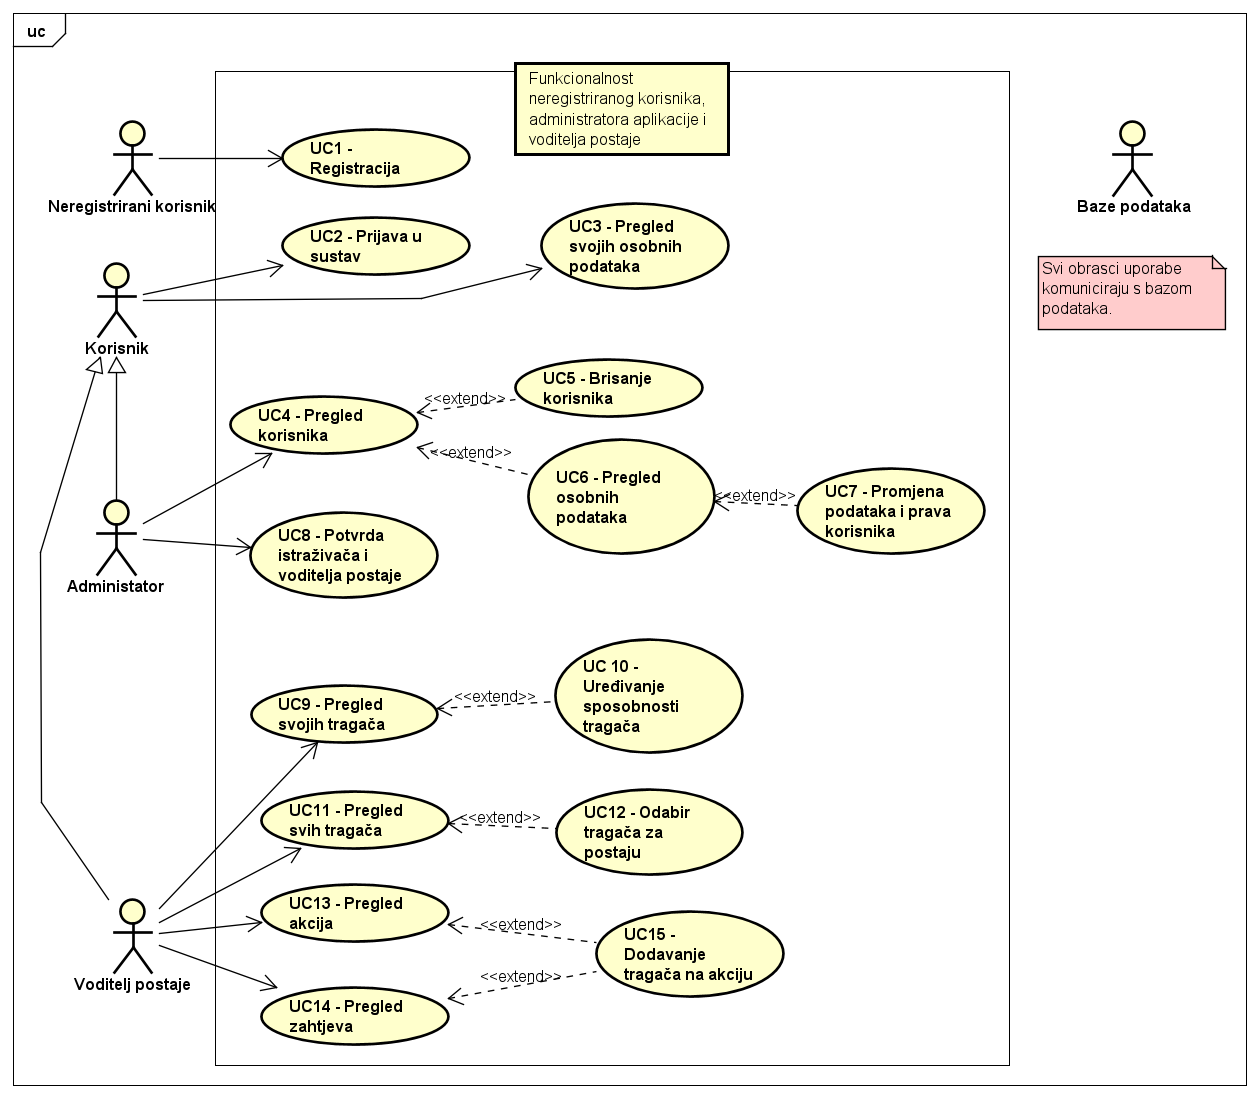
\includegraphics[scale=0.8]{slike/dijagram admin.png} %veličina slike u odnosu na originalnu datoteku i pozicija slike
						\centering
						\caption{Funkcionalnost neregistriranog korisnika, generaliziranog korisnika, administratora aplikacije i voditelja postaje}
						\label{fig:Funkcionalnost neregistriranog korisnika, administratora aplikacije i voditelja postaje}
					\end{figure}
					
					\begin{figure}[H]
						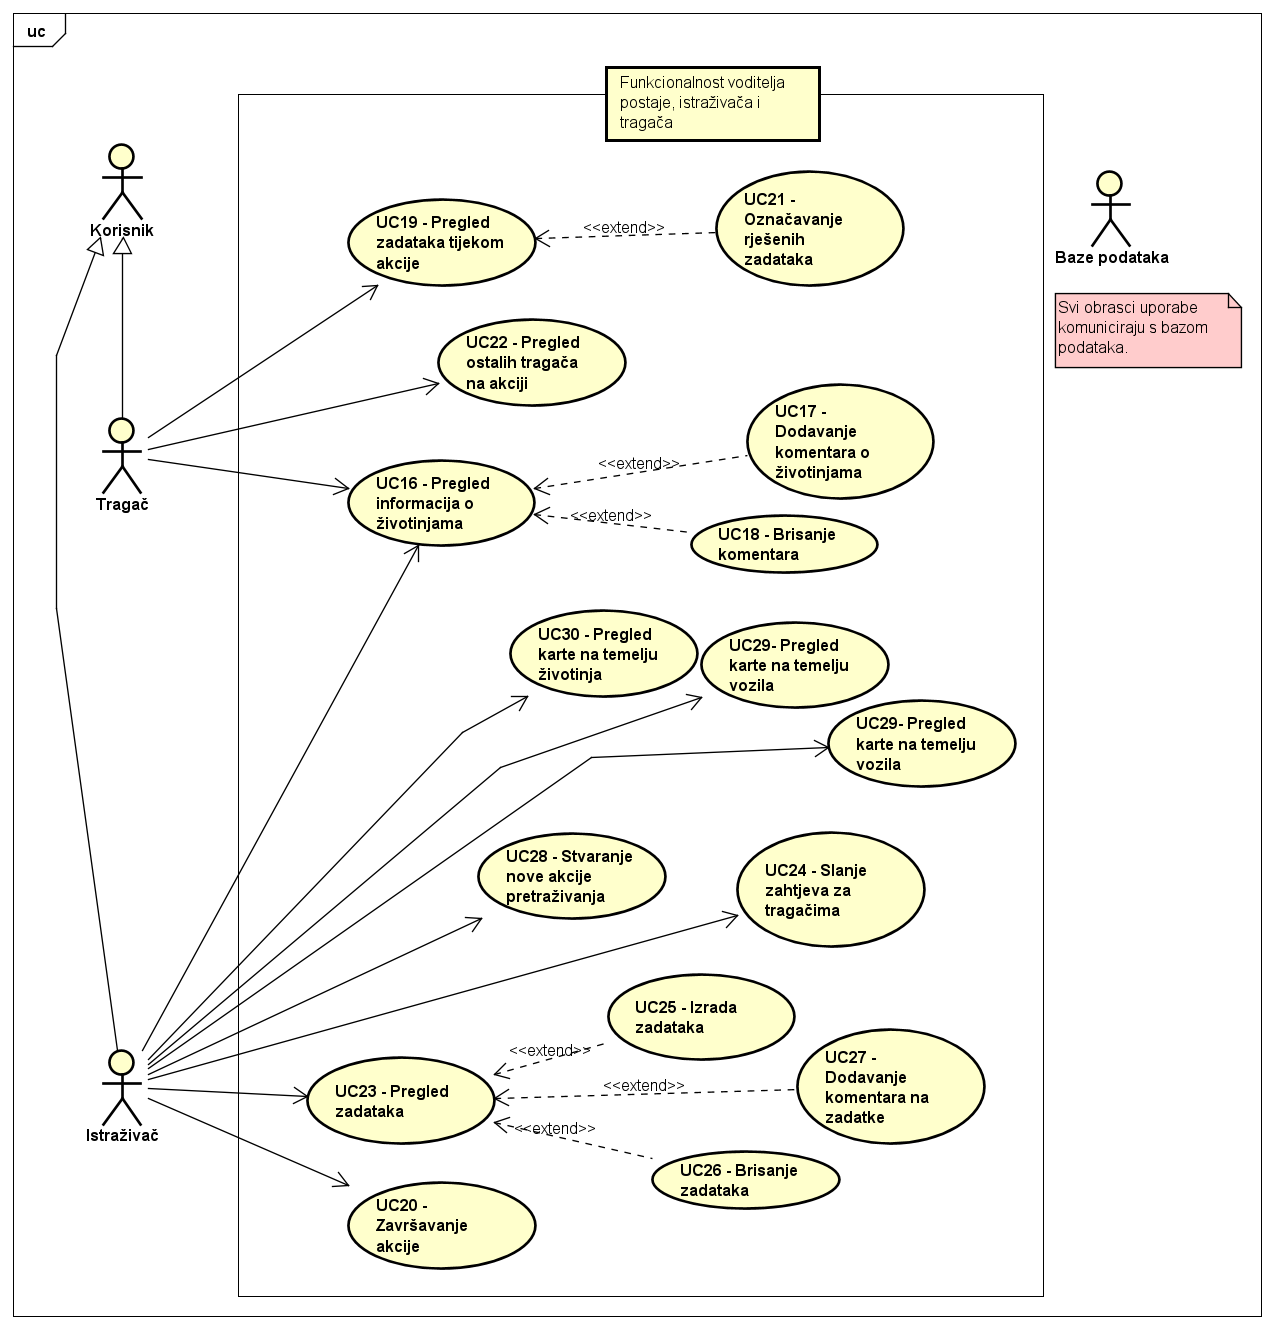
\includegraphics[scale=0.8]{slike/dijagram ekipa.png} %veličina slike u odnosu na originalnu datoteku i pozicija slike
						\centering
						\caption{Funkcionalnost tragača i istraživača}
						\label{fig:Funkcionalnost tragača i istraživača}
					\end{figure}
				
					\eject		
				
			\subsection{Sekvencijski dijagrami}
				
				\noindent 
				\textbf{Obrazac uporabe UC1 - Registracija}\\

				\noindent 
				Neregistrirani korisnik šalje zahtjev za registracijom. Aplikacija dohvaća popis registriranih korisnika
        				iz baze podataka.
        				Ako korisnik nije na popisu aplikacija mu šalje potvrdu na mail koju korisnik mora potvrditi.
        				U slučaju da se korisnik registrira da bi bio voditelj postaje ili istraživač aplikacija šalje administratoru
        				zahtjev za potvrdom te administrator mora potvrditi registraciju.
        				Zatim aplikacija zapisuje podatke u bazu podataka te dobiva potvrdu o uspjehu registracije od baze podataka
        				te aplikacija korisniku prikazuje poruku o uspješnoj registraciji.
        				Ako korisnik postoji u bazi podataka aplikacija, korisnik se obavještava da korisnik već postoji u bazi podataka.

				
				
				\begin{figure}[H]
					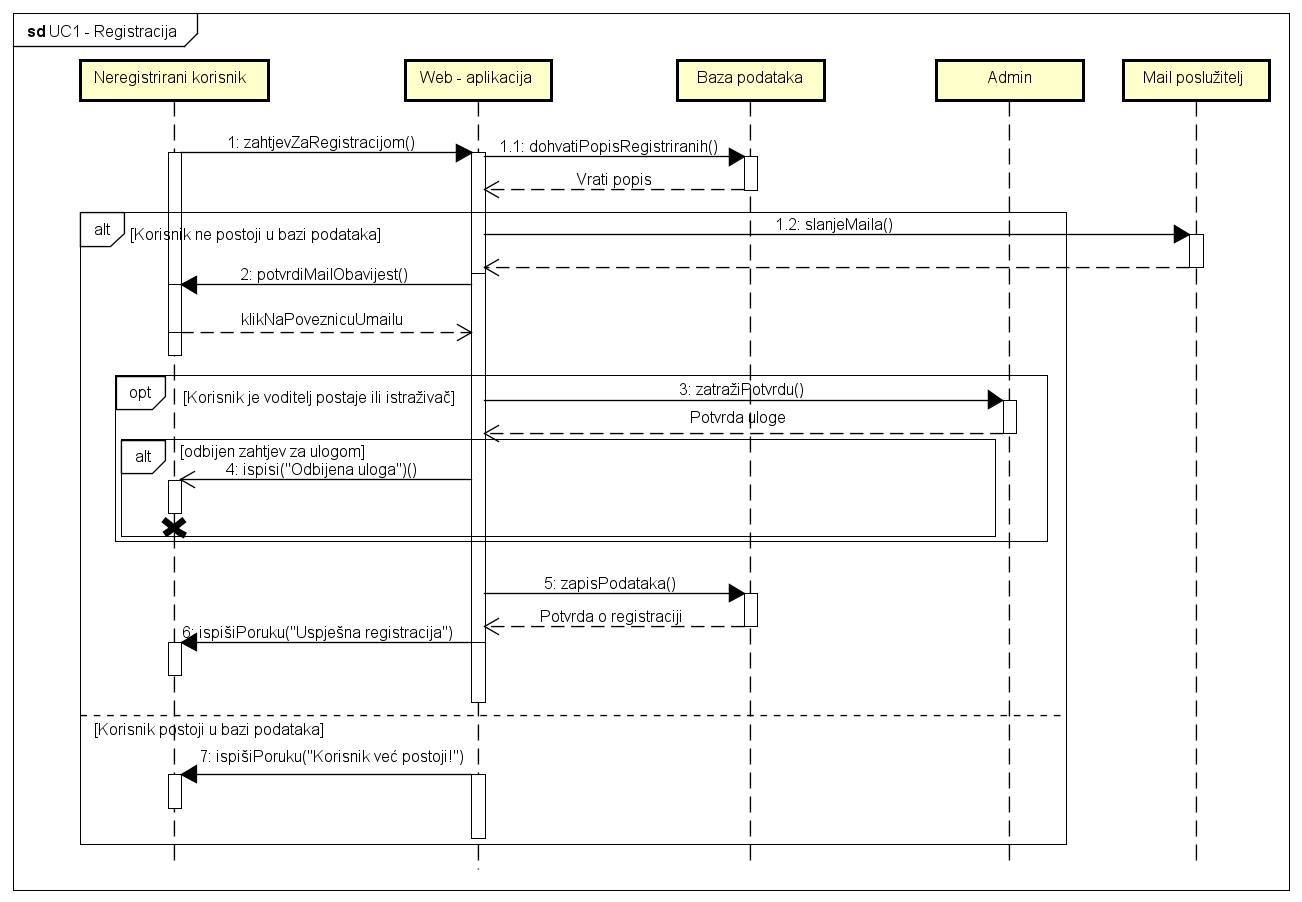
\includegraphics[scale=0.5]{slike/UC1 - Registracija.png} %veličina slike u odnosu na originalnu datoteku i pozicija slike
					\centering
					\caption{Sekvencijski dijagram za UC1}
					\label{fig:UC1 - Registracija}
				\end{figure}

				\eject

				\noindent
				\textbf{Obrazac uporabe UC19 - Dodavanje tragača na akciju}\\

				\noindent
				Voditelj postaje šalje aplikaciji upit za novim akcijama.
        			Aplikacija dohvaća popis aktivnih akcija iz baze podataka te ih prikazuje voditelju postaje.
        			Voditelj postaje zatim prolazi kroz sve aktivne akcije.
        			Aplikacija iz baze podataka dohvaća sve slobodne tragače koji zadovoljavaju zahtjeve istraživača.
        			U slučaju da ne postoje takvi tragači voditelju se postaje ispisuje poruka da nema dostupnih tragača.
        			U slučaju da popis nije prazan voditelju postaje prikazuje se popis tragača.
        			Voditelj postaje potom šalje odabrane tragače aplikaciji koja zatim dodaje akciju tragaču u bazi podataka te
        			vraća voditelju postaje obavijest da je zahtjev poslan tragaču.

				

				\begin{figure}[H]
					\includegraphics[scale=0.5]{slike/UC19 - Dodavanje tragača na akciju.png} %veličina slike u odnosu na originalnu datoteku i pozicija slike
					\centering
					\caption{Sekvencijski dijagram za UC19}
					\label{fig:UC19 - Dodavanje tragača na akciju}
				\end{figure}
	
				\eject

				\noindent
				\textbf{Obrazac uporabe UC24 - Završavanje akcije}\\

				\noindent
				Tragač šalje aplikaciji zahtjev za krajem akcije.
        				Aplikacija dohvaća popis zadataka iz baze podataka i prikazuje popis tragaču.
        				Ako popis nije prazan tragaču se ispisuje poruka da nisu svi zadatci riješeni.
				        Ako je popis prazan aplikacija šalje bazi podataka zahtjev za krajem akcije
        				te potom obavještava tragača da je akcija završena.

				

				\begin{figure}[H]
					\includegraphics[scale=0.6]{slike/UC24 - Završavanje akcije.png} %veličina slike u odnosu na originalnu datoteku i pozicija slike
					\centering
					\caption{Sekvencijski dijagram za UC24}
					\label{fig:UC24 - Završavanje akcije}
				\end{figure}

				\eject

				\noindent
				\textbf{Obrazac uporabe UC37 - Stvaranje nove akcije pretraživanja}\\

				\noindent
				Istraživač aplikaciji šalje zahtjev za novom akcijom.
				        Aplikacija provjerava ima li istraživač već aktivne akcije.
        				U slučaju da istraživač već ima aktivnu akciju aplikacija obavještava istraživača da već postoji aktivna akcija.
        				Ako istraživač nema aktivnu akciju aplikacija bazi podataka šalje zahtjev za dodavanjem nove akcije te se
        				istraživač obavještava da je akcija uspješno stvorena.

				

				\begin{figure}[H]
					\includegraphics[scale=0.5]{slike/UC37 - Stvaranje nove akcije pretraživanja.png} %veličina slike u odnosu na originalnu datoteku i pozicija slike
					\centering
					\caption{Sekvencijski dijagram za UC37}
					\label{fig:UC37 - Stvaranje nove akcije pretraživanja}
				\end{figure}

				\eject
	
		\section{Ostali zahtjevi}

		\begin{packed_item}
			\item Sustav treba podržavati istovremeni rad više korisnika u stvarnom vremenu
			\item Korisničko sučelje i sustav moraju podržavati hrvatsku abecedu 
			\item Pristup bazi podataka trebao bi biti učinkovit, s vremenom izvršavanja unutar nekoliko sekundi
			\item Za izradu sustava kao web aplikacije, koriste se objektno-orijentirani jezici
			\item Pogrešna uporaba korisničkog sučelja ne bi smjela imati negativan utjecaj na funkcionalnost i rad sustava
			\item Sustav treba biti jednostavan za korištenje
			\item Pri nadogradnji sustava, ne smiju se narušavati postojeće funkcionalnosti
			\item Veza s bazom podataka mora biti zaštićena, brza i otporna na vanjske greške
			\item Pristup sustavu treba biti moguć iz javne mreže, uz korištenje HTTPS-a radi sigurne komunikacije
		\end{packed_item}
	
	\chapter{Arhitektura i dizajn sustava}

Arhitektura sustava može se podijeliti na tri ključna podsustava:

\begin{packed_enum}
	\item Web poslužitelj:
	\begin{packed_enum}
		\item Ključan dio web aplikacije.
		\item Odgovoran za interakciju između klijenta i aplikacije.
		\item Koristi HTTP/HTTPS protokol za prijenos informacija na webu.
		\item Inicira pokretanje web aplikacije i proslijeđuje zahtjeve.
	\end{packed_enum}
	\item Web aplikacija:
	\begin{packed_enum}
		\item Procesira korisničke zahtjeve i obrađuje ih.
		\item Pristupa bazi podataka prema potrebi.
		\item Generira odgovore u obliku HTML dokumenata za prikaz u web pregledniku.
	\end{packed_enum}			
	\item Baza podataka:	
	\begin{packed_enum}
		\item Sprema podatke koji se koriste ili modificiraju unutar web aplikacije.
	\end{packed_enum}
\end{packed_enum}

Korisnik, putem web preglednika, šalje zahtjeve web poslužitelju. 
Web poslužitelj zatim inicira rad web aplikacije, koja procesira zahtjeve, pristupa bazi podataka po potrebi i vraća odgovore u obliku HTML dokumenata. 
Ova interakcija omogućuje korisnicima pregled i manipulaciju sadržajem putem web sučelja.

\begin{figure}[H]
	\includegraphics[scale=0.5]{slike/arhitektura.png}
	\centering
	\caption{Arhitektura sustava}
	\label{fig:arhitektura}
\end{figure}

Za izradu ovog projekta koristili smo se Spring Boot frameworkom u Javi kroz
razvojno okruženje IntelliJ Community Edition, Javascriptom uz React u Visual
Studio Code-u te drugim programima za dizajn slika i grafova ( AstahUML itd.).


 Spring Boot podržava koncept MVC, odnosno Model-Pogled-Nadglednik
(engl. \textit{Model View Controller}), arhitekture, tj. stilističke varijacije arhitekture zasnovane 
na događajima. Takve arhitekture odlikuje to što se komponente međusobno ne pozivaju
eksplicitno, već neke od njih generiraju signale (događaje) ne znajući koja druga
"osluškuje" tj. očekuje takav signal i na njega reagira. To se postiže kroz Spring Web MVC modul. 
\begin{packed_item}
	\item Model: Spring Boot omogućava korištenje Java objekata kao modela. Ovi objekti predstavljaju podatke koji se koriste u aplikaciji.
	Spring Data može se integrirati za jednostavno upravljanje podacima i komunikaciju s bazom podataka.
	\item View: Spring Boot pruža fleksibilnost u odabiru tehnologije za prikazivanje korisničkog sučelja. Prikazi se često implementiraju kroz HTML datoteke, a moguće je koristiti različite template engines (Thymeleaf, FreeMarker, JSP).
	Pomoću konfiguracija view resolvera jednostavno se integriraju odabrane tehnologije za prikazivanje podataka korisnicima.
	\item Controller: Anotacije poput @Controller i @RestController omogućuju jednostavno označavanje klasa koje djeluju kao kontroleri.
	@RequestMapping i slične anotacije omogućuju mapiranje HTTP zahtjeva na određene metode kontrolera.
	Spring Boot automatski prepoznaje i konfigurira komponente kontrolera.		
\end{packed_item}

Kod MVC-a pogodno je što smanjuje međuovisnost korisničkog sučelja i ostatka sustava, a omogućuje i nezavisan razvoj, nadogradnje i dodavanje različitih dijelova aplikacije. Sadrži različite
gotove predloške za klase koji nam olakšavaju proces izrade.
				
		\section{Baza podataka}
			    


		Baze podataka neizostavan su dio razvoja programske potpore jer danas gotova svaka domena primjene 
		obiluje mnoštvom podataka koje treba pohraniti na organiziran način kako bi se efikasno dohvaćali,
		 mijenjali i nadopunjavali. Za upravljanje bazom podataka mogu se koristiti različiti sustavi koji 
		 obavljaju optimiranje upita i omogućuju rukovanje podatcima. Mi smo odlučili koristiti PostgreSQL 
		 koji nam je bio preporučen na kolegiju Baze podataka. \newline Relacijski nam model baze podataka 
		 omogućuje vjeran prikaz stvarnosti pomoću relacija u koje pohranjujemo vrijednosti odabranih 
		 atributa vezanih uz entitete bitne za domenu primjene. Atributi su imenovani stupci te tablice. ER (Entity-Relationship) model podataka zadržava dobra svojstva relacijskog modela, a uz to omogućuje eksplicitni prikaz semantičkih informacija vezanih uz veze (odnose) između entiteta. Kako bismo prikazali kako su eniteti našeg sustava povezani koristit ćemo ER model baze podataka.
za podataka ove aplikacije sastoji se od sljedećih entiteta:
		\begin{packed_item}
			\item Korisnik
			\item Pozicija tragača
			\item Uloga
			\item Zadatak 
			\item Pripada postaji
			\item Osposobljen za
			\item Akcija
			\item Postaja
			\item Prijevozno sredstvo
			\item Komentar korisnika 
			\item Životinja
			\item Pozicija životinje
		\end{packed_item}

		\eject
			\subsection{Opis tablica}
			
					\textbf {Zadatak} Ovaj entitet sadrži sve važne informacije o zadatcima koje obavljaju tragači tijekom akcije, a stvaraju istraživači. Sadrži
				atribute: šifra zadatka, korisničko ime, tekst, završen, šifra akcije, šifra životinje i šifra vozila. 
				Ova tablica je u vezi s tablicom Prijevozno sredstvo preko tablice Osposobljen za te izravno preko 
				dentifikatora vozila(šifra vozila), s tablicom Akcija izravno preko identifikatora akcije (šifra akcije), 
				s tablicom Životinja izravno preko identifikatora životinje (šifra životinje).
				
				\begin{longtblr}[
					label=none,
					entry=none
					]{
						width = \textwidth,
						colspec={|X[6,l]|X[6, l]|X[20, l]|}, 
						rowhead = 1,
					} %definicija širine tablice, širine stupaca, poravnanje i broja redaka naslova tablice
					\hline \SetCell[c=3]{c}{\textbf{Zadatak}}	 \\ \hline[3pt]
					\SetCell{LightGreen} Šifra Zadatka & INT	&  	Jedinstveni brojčani identifikator zadatka  	\\ \hline
					\SetCell{LightGreen} Korisničko ime & VARCHAR	& 	Korisničko ime korisnika\\ \hline
					Tekst	& VARCHAR & Opis zadatka  	\\ \hline 
					Završen & BOOLEAN & Status je li zadatak završen  \\ \hline 
          \SetCell{LightBlue} Šifra akcije 	& INT & Jedinstveni brojčani identifikator akcije   	\\ \hline 
          \SetCell{LightBlue} Šifra životinje 	& INT &   Jedinstveni brojčani identifikator životinje  	\\ \hline 
          \SetCell{LightBlue} Šifra vozila 	& INT &  Jedinstveni brojčani identifikator vozila 	\\ \hline 
				\end{longtblr}

				\textbf {Akcija} Ovaj entitet sadrži sve važne informacije o akcijama pretraživanja i praćenja. Sadrži
			atribute: šifra akcije, naziv akcije, aktivna i korisničko ime. 
			Ova tablica je u vezi s tablicom Korisnik preko identifikatora korisnika(korisničko ime),
			 s tablicom Životinja preko tablice Komentar korisnika, s tablicom Zadatak i tablicom Pozicija tragača.
				
				\begin{longtblr}[
					label=none,
					entry=none
					]{
						width = \textwidth,
						colspec={|X[6,l]|X[6, l]|X[20, l]|}, 
						rowhead = 1,
					} %definicija širine tablice, širine stupaca, poravnanje i broja redaka naslova tablice
          \hline \SetCell[c=3]{c}{\textbf{Akcija}}	 \\ \hline[3pt]
					\SetCell{LightGreen} Šifra akcije & INT	&  	Jedinstveni ključ za identifikaciju zadatka  	\\ \hline
					Naziv akcije	& VARCHAR &  Puni naziv akcije  	\\ \hline 
					Aktivna & BOOLEAN & Status je li akcija aktvna  \\ \hline 
          \SetCell{LightBlue} Korisničko ime 	& VARCHAR &  Korisničko ime korisnika 	\\ \hline 
				\end{longtblr}
			
				\textbf {Komentar korisnika} Ovaj entitet sadrži informacije o komentarima korisnika o praćenoj životinji 
				koje mogu ostaviti tijekom akcije. Sadrži atribute: šifra životinje, korisničko ime, šifra akcije i komentar. 
		

				\begin{longtblr}[
					label=none,
					entry=none
					]{
						width = \textwidth,
						colspec={|X[6,l]|X[6, l]|X[20, l]|}, 
						rowhead = 1,
					} %definicija širine tablice, širine stupaca, poravnanje i broja redaka naslova tablice
          \hline \SetCell[c=3]{c}{\textbf{Komentar korisnika}}	 \\ \hline[3pt]
					\SetCell{LightGreen} Šifra životinje & INT	&  	Jedinstveni brojčani identifikator zadatka  	\\ \hline
					\SetCell{LightGreen} Korisničko ime & VARCHAR	&  	Korisničko ime korisnika 	\\ \hline
					\SetCell{LightGreen} Šifra akcije & INT	&  	Jedinstveni brojčani identifikator akcije  	\\ \hline
					Komentar	& VARCHAR & Sadržaj komentara  	\\ \hline 
				\end{longtblr}
				
				\textbf {Životinja} Ovaj entitet sadrži sve važne informacije o životinjama. Sadrži
			atribute: šifra životinje, naziv , latinski naziv i opis. 
			Ova tablica povezana je s tablicom Pozicija životinje s tablicom Zadatak preko identifikatora životinje(šifra životinje) te s tablicom Akcija

				\begin{longtblr}[
					label=none,
					entry=none
					]{
						width = \textwidth,
						colspec={|X[6,l]|X[6, l]|X[20, l]|}, 
						rowhead = 1,
					} %definicija širine tablice, širine stupaca, poravnanje i broja redaka naslova tablice
          \hline \SetCell[c=3]{c}{\textbf{Životinja}}	 \\ \hline[3pt]
					\SetCell{LightGreen} Šifra životinje & INT	&  	Jedinstveni brojčani identifikator životinje  	\\ \hline
					Naziv	& VARCHAR & Puni naziv životinje  	\\ \hline 
					Latinski naziv	& VARCHAR & Latinski naziv životinje  	\\ \hline 
					Opis	& VARCHAR & Sadržaj komentara  	\\ \hline 
				\end{longtblr}

				\textbf {Pozicija životinje} Ovaj entitet sadrži informacije o poziciji životinje. 
				Pomoću njega bilježimo gibanje životinje na kartama. Sadrži
			atribute: šifra životinje, vremenska oznaka, geografska širina i geografska dužina.


				\begin{longtblr}[
					label=none,
					entry=none
					]{
						width = \textwidth,
						colspec={|X[6,l]|X[6, l]|X[20, l]|}, 
						rowhead = 1,
					} %definicija širine tablice, širine stupaca, poravnanje i broja redaka naslova tablice
          \hline \SetCell[c=3]{c}{\textbf{Pozicija životinje}}	 \\ \hline[3pt]
					\SetCell{LightGreen} Šifra životinje & INT	&  	Jedinstveni brojčani identifikator životinje \\ \hline
					\SetCell{LightGreen} Vremenska oznaka & TIMESTAMP	&  	Zadnje vrijeme u kojem je viđena životinja  	\\ \hline
          Geografska širina	& DOUBLE & Iznos geografske širine  	\\ \hline 
          Geografska dužina	& DOUBLE & Iznos geografske dužine  	\\ \hline 
				\end{longtblr}

				\textbf {Pozicija tragača} Ovaj entitet sadrži informacije o poziciji tragača. 
				Pomoću njega bilježimo kretanje tragača na kartama. Sadrži
			atribute: korisničko ime, vremenska oznaka, šifra akcije, geografska širina i geografska dužina.

				\begin{longtblr}[
					label=none,
					entry=none
					]{
						width = \textwidth,
						colspec={|X[6,l]|X[6, l]|X[20, l]|}, 
						rowhead = 1,
					} %definicija širine tablice, širine stupaca, poravnanje i broja redaka naslova tablice
          \hline \SetCell[c=3]{c}{\textbf{Pozicija tragača}}	 \\ \hline[3pt]
					\SetCell{LightGreen} Korisničko ime & VARCHAR	&  	Korisničko ime korisnika  	\\ \hline
					\SetCell{LightGreen} Vremenska oznaka & TIMESTAMP	&  	Zadnje vrijeme kada je tragač zabilježio svoju poziciju  	\\ \hline
					\SetCell{LightGreen} Šifra akcije & INT	&  	Jedinstveni brojčani identifikator akcije  	\\ \hline
          Geografska širina	& DOUBLE & Iznos geografske širine  	\\ \hline 
          Geografska dužina	& DOUBLE & Iznos geografske dužine  	\\ \hline 
				\end{longtblr}

				\textbf {Korisnik} Ovaj entitet sadrži sve važne informacije o korisnicima. Sadrži
			atribute: korisničko ime, email, lozinka, ime, prezime, fotografija i šifra uloge.
			Ova tablica je u vezi s tablicama Akcija, Pozicija tragača, Uloga i Komentar korisnika.

				\begin{longtblr}[
					label=none,
					entry=none
					]{
						width = \textwidth,
						colspec={|X[6,l]|X[6, l]|X[20, l]|}, 
						rowhead = 1,
					} %definicija širine tablice, širine stupaca, poravnanje i broja redaka naslova tablice
          \hline \SetCell[c=3]{c}{\textbf{Korisnik}}	 \\ \hline[3pt]
					\SetCell{LightGreen} Korisničko ime & VARCHAR	&  	Ime korisnika  	\\ \hline
          Email	& VARCHAR & Sadržaj komentara  	\\ \hline 
          Lozinka & VARCHAR & Lozinka korisnika \\ \hline
          Ime & VARCHAR & Ime korisnika \\ \hline
          Prezime & VARCHAR & Prezime korisnika \\ \hline
          Fotografija & VARCHAR & Fotografija korisnika \\ \hline
          \SetCell{LightBlue} Šifra uloge 	& INT &   Jedinstveni brojčani identifikator uloge	\\ \hline 

				\end{longtblr}

				\textbf {Pripada postaji} Ova veza sadrži informacije po kojima saznajemo koji korisnik pripada kojoj postaji.
				Povezuje entitete Korisnik i Postaja te sadrži njihove ključne atribute: korisničko ime i šifra postaje.

				\begin{longtblr}[
					label=none,
					entry=none
					]{
						width = \textwidth,
						colspec={|X[6,l]|X[6, l]|X[20, l]|}, 
						rowhead = 1,
					} %definicija širine tablice, širine stupaca, poravnanje i broja redaka naslova tablice
          \hline \SetCell[c=3]{c}{\textbf{Pripada postaji}}	 \\ \hline[3pt]
					\SetCell{LightGreen} Korisničko ime & VARCHAR	&  	Korisničko ime korisnika  	\\ \hline
					\SetCell{LightGreen} Šifra postaje & VARCHAR	&  	Jedinstveni brojčani identifikator postaje\\ \hline

				\end{longtblr}

				\textbf {Postaja} Ovaj entitet sadrži informacije o postajama. Sastoji se od
			atributa: šifra postaje i naziv postaje.

				\begin{longtblr}[
					label=none,
					entry=none
					]{
						width = \textwidth,
						colspec={|X[6,l]|X[6, l]|X[20, l]|}, 
						rowhead = 1,
					} %definicija širine tablice, širine stupaca, poravnanje i broja redaka naslova tablice
          \hline \SetCell[c=3]{c}{\textbf{Postaja}}	 \\ \hline[3pt]
					\SetCell{LightGreen} Šifra postaje & VARCHAR	&  	Jedinstveni brojčani identifikator korisnika \\ \hline
					Naziv postaje & VARCHAR	&  	Pun naziv postaje  	\\ \hline

				\end{longtblr}

				\textbf {Osposobljen za} Ova veza sadrži informacije po kojima saznajemo koji korisnik ima sposobnosti za voziti koje prijevozno sredstvo.
				Povezuje entitete Korisnik i Prijevozno sredstvo te sadrži njihove ključne atribute: korisničko ime i šifra vozila.

				\begin{longtblr}[
					label=none,
					entry=none
					]{
						width = \textwidth,
						colspec={|X[6,l]|X[6, l]|X[20, l]|}, 
						rowhead = 1,
					} %definicija širine tablice, širine stupaca, poravnanje i broja redaka naslova tablice
          \hline \SetCell[c=3]{c}{\textbf{Osposobljen za}}	 \\ \hline[3pt]
					\SetCell{LightGreen} Korisničko ime & VARCHAR	&  	Ime korisnika  	\\ \hline
					\SetCell{LightGreen} Šifra vozila & INT	&   Jedinstveni brojčani identifikator vozila  	\\ \hline

				\end{longtblr}

				\textbf {Prijevozno sredstvo} Ovaj entitet sadrži informacije o vozilima za koje tragači mogu biti osposobljeni.
				 Sastoji se od atributa: šifra vozila i naziv vozila.


				\begin{longtblr}[
					label=none,
					entry=none
					]{
						width = \textwidth,
						colspec={|X[6,l]|X[6, l]|X[20, l]|}, 
						rowhead = 1,
					} %definicija širine tablice, širine stupaca, poravnanje i broja redaka naslova tablice
          \hline \SetCell[c=3]{c}{\textbf{Prijevozno sredstvo}}	 \\ \hline[3pt]
					\SetCell{LightGreen} Šifra vozila & INT	&   Jedinstveni brojčani identifikator vozila  	\\ \hline
          Naziv vozila & VARCHAR & Puni naziv vozila \\ \hline

				\end{longtblr}

				\textbf {Uloga} Ovaj entitet sadrži informacije o ulogama korisnika. Sastoji se od
			atributa: šifra uloge i naziv uloge.


				\begin{longtblr}[
					label=none,
					entry=none
					]{
						width = \textwidth,
						colspec={|X[6,l]|X[6, l]|X[20, l]|}, 
						rowhead = 1,
					} %definicija širine tablice, širine stupaca, poravnanje i broja redaka naslova tablice
          \hline \SetCell[c=3]{c}{\textbf{Uloga}}	 \\ \hline[3pt]
          \SetCell{LightGreen} Šifra Uloge & INT	&  Jedinstveni brojčani identifikator uloge	\\ \hline
          Naziv uloge	& VARCHAR & Puni naziv uloge  	\\ \hline 

				\end{longtblr}

			\eject

			\subsection{Dijagram baze podataka}

			\begin{figure}[H]
				\includegraphics[scale=0.9]{slike/dijagram baze podataka.png} 
				\centering
				\caption{Dijagram baze podataka}
				\label{fig:dijagram_baze_podataka}
			\end{figure}
			
			\eject
			
			
		\section{Dijagram razreda}

		Na slikama \ref{fig:controllers}, \ref{fig:data_transfer_objects} i \ref{fig:models} su prikazani klasni dijagrami koji pripadaju backend dijelu MVC
		arhitekture. Razredi prikazani na slici \ref{fig:controllers} nasljeđuju Controller razred. 
		Metode implementirane u tim razredima manipuliraju s Data transfer object, a oni
		su dohvaćeni s pomoću metoda u Model razredima. 

		Metode unutar Controller razreda vraćaju JSON datoteke s odgovarajućim html status kodom.
		Razredi su logički podijeljeni prema pravu pristupa metodama specifičnih aktora kako bi se smanjila prenapučenost unutar dijagrama.
		Pri prikazu su naglašene samo ovisnosti između razreda koji pripadaju istom dijelu dijagrama radi jednostavnije organizacije.
		Vrsta ovisnosti između različitim razredima može se zaključiti iz naziva i tipova atributa unutar tih razreda.
		
		\eject

			\begin{figure}[H]
				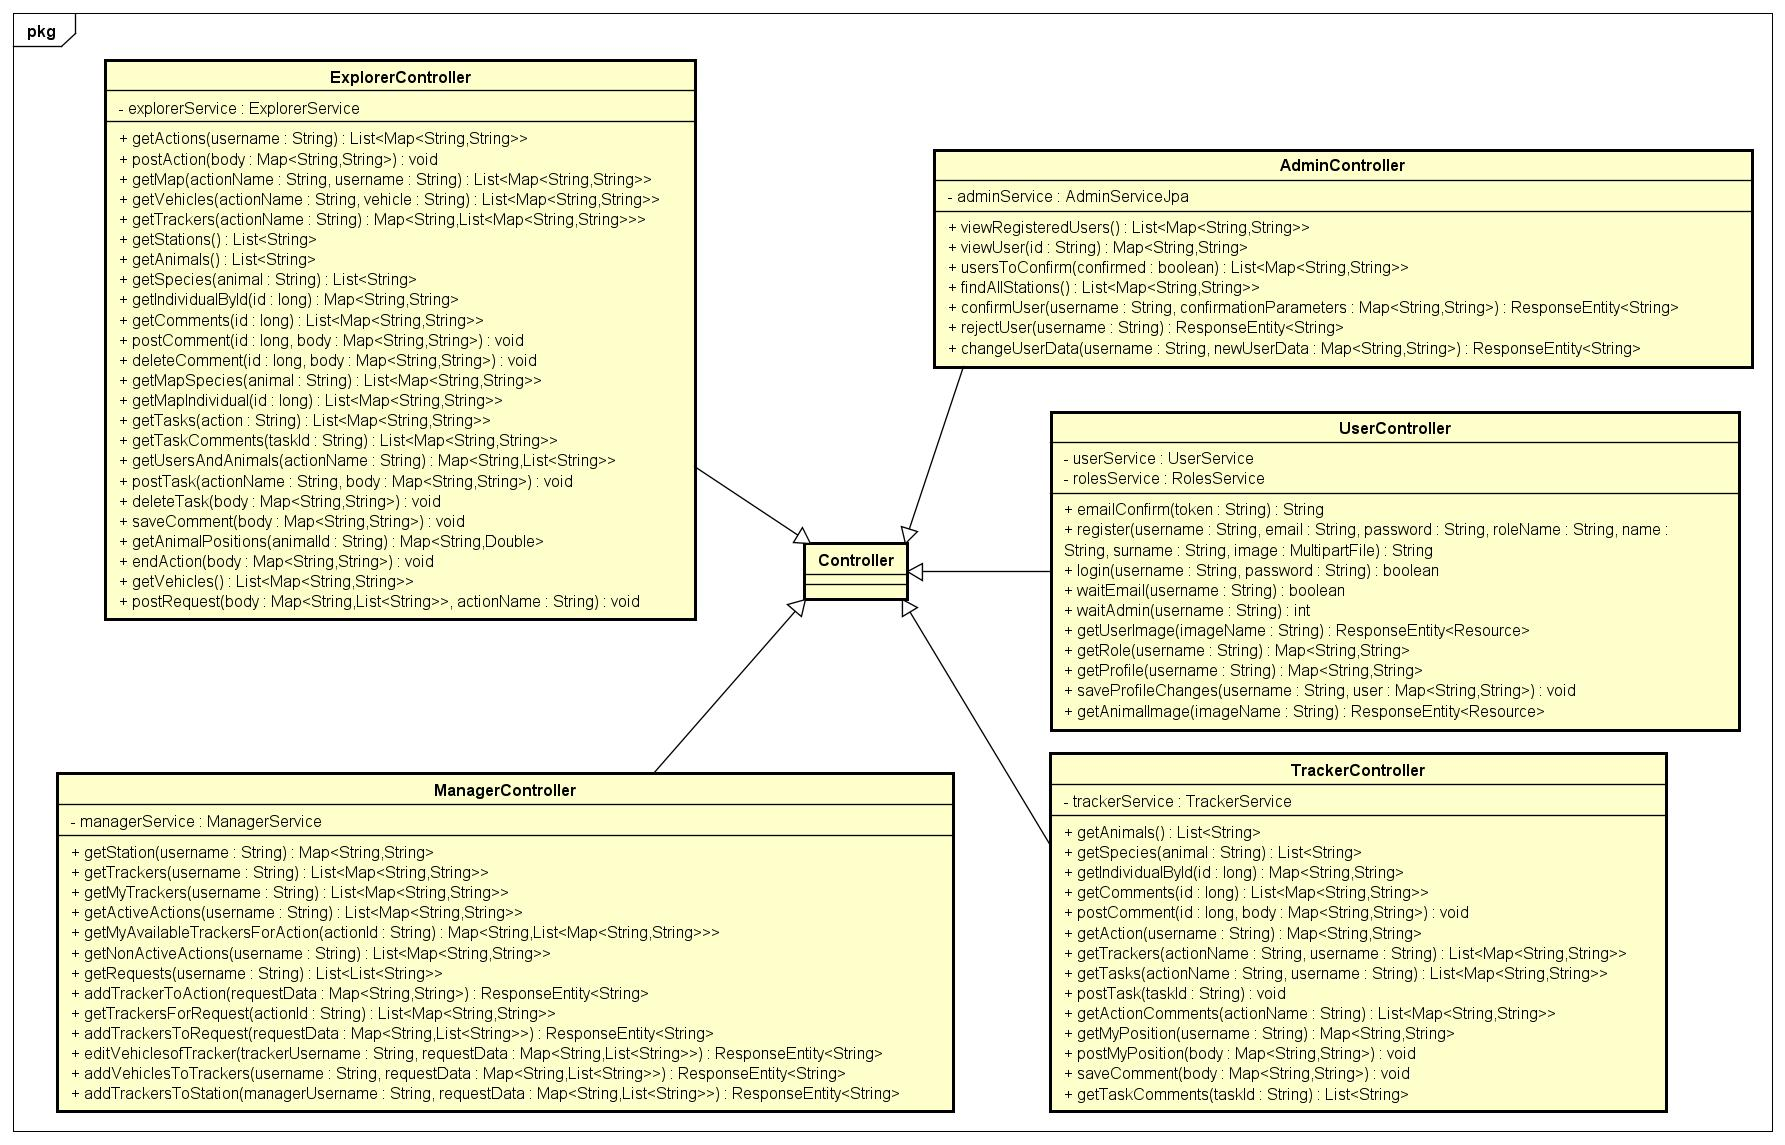
\includegraphics[scale=0.4]{slike/klasni_dijagram_controllers.jpg}
				\centering
				\caption{Dijagram razreda - dio Controllers}
				\label{fig:controllers}
			\end{figure}
			
			\eject

			\begin{figure}[H]
				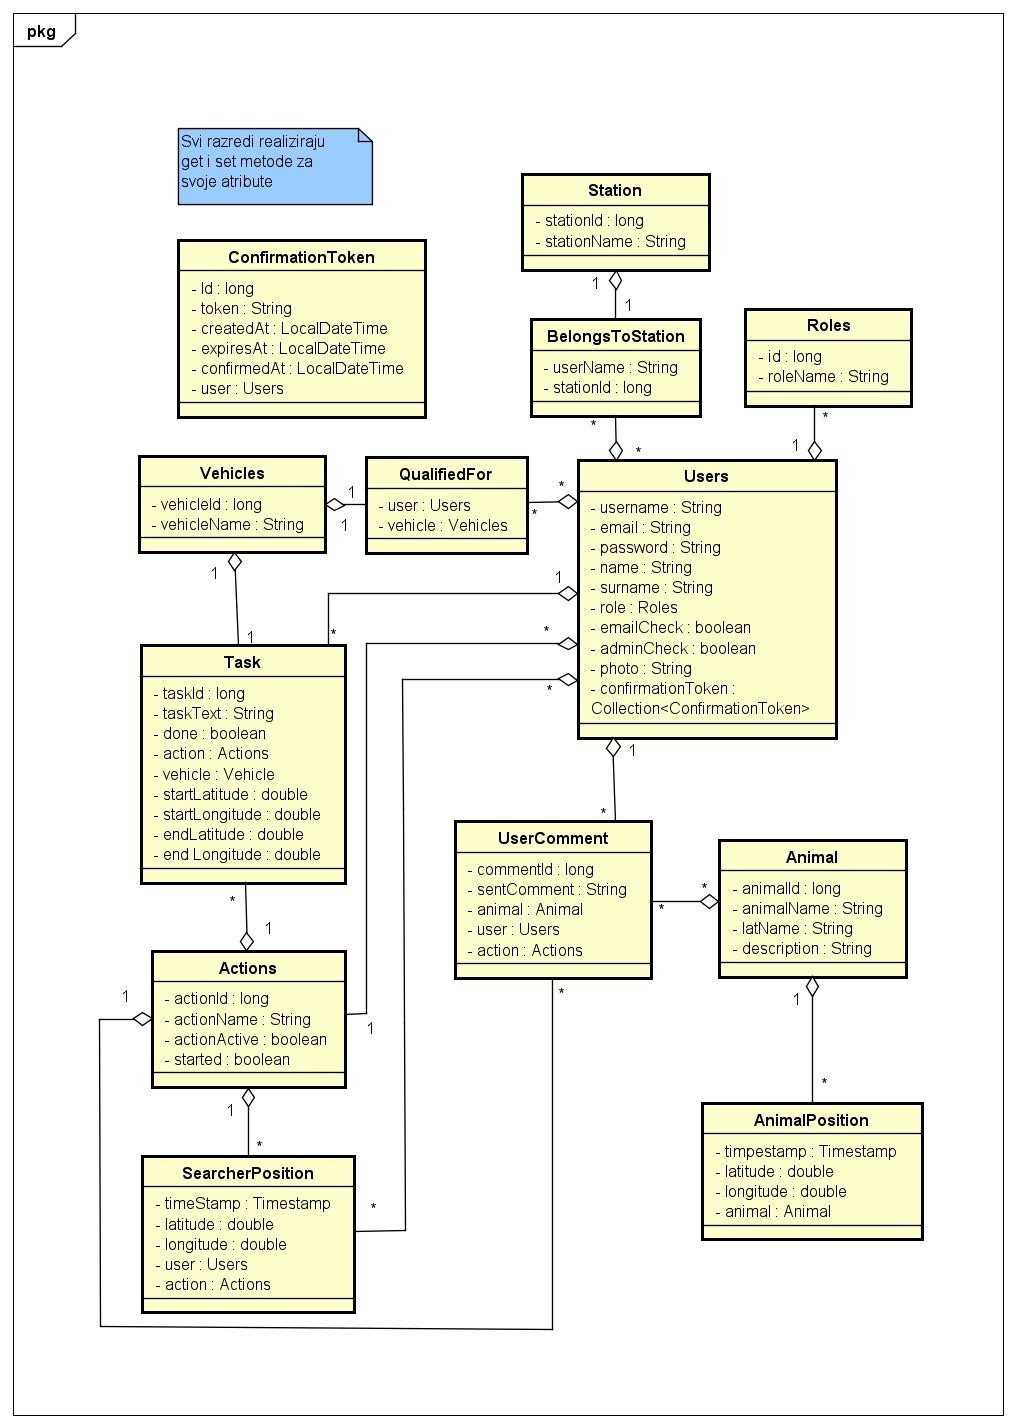
\includegraphics[scale=0.5]{slike/klasni_dijagram_DTO.jpg}
				\centering
				\caption{Dijagram razreda - dio Data transfer objects}
				\label{fig:data_transfer_objects}
			\end{figure}

			Model razredi prikazuju strukturu baze podataka u aplikaciji. 
			Implementirane metode komuniciraju s bazom podataka te vraćaju tražene podatke. 
			Razred Users predstavlja neregistriranog korisnika koji se može registrirati u 
			sustav unošenjem informacija. Razred Administrator predstavlja administratora 
			sustava koji ima najveće ovlasti. Razred Leader predstavlja voditelja postaje koji ima mogućnost postavljanja tragača određenom istraživaču.
			Razred Researcher predstavlja istraživača koji ima pristup karti tragača i životinja te može tragaču zadati zadatak. 
			Razred Searcher predstavlja tragača koji ima pristup karti životinja te može ispunjavati zadatke.


			\eject

			\begin{figure}[H]
				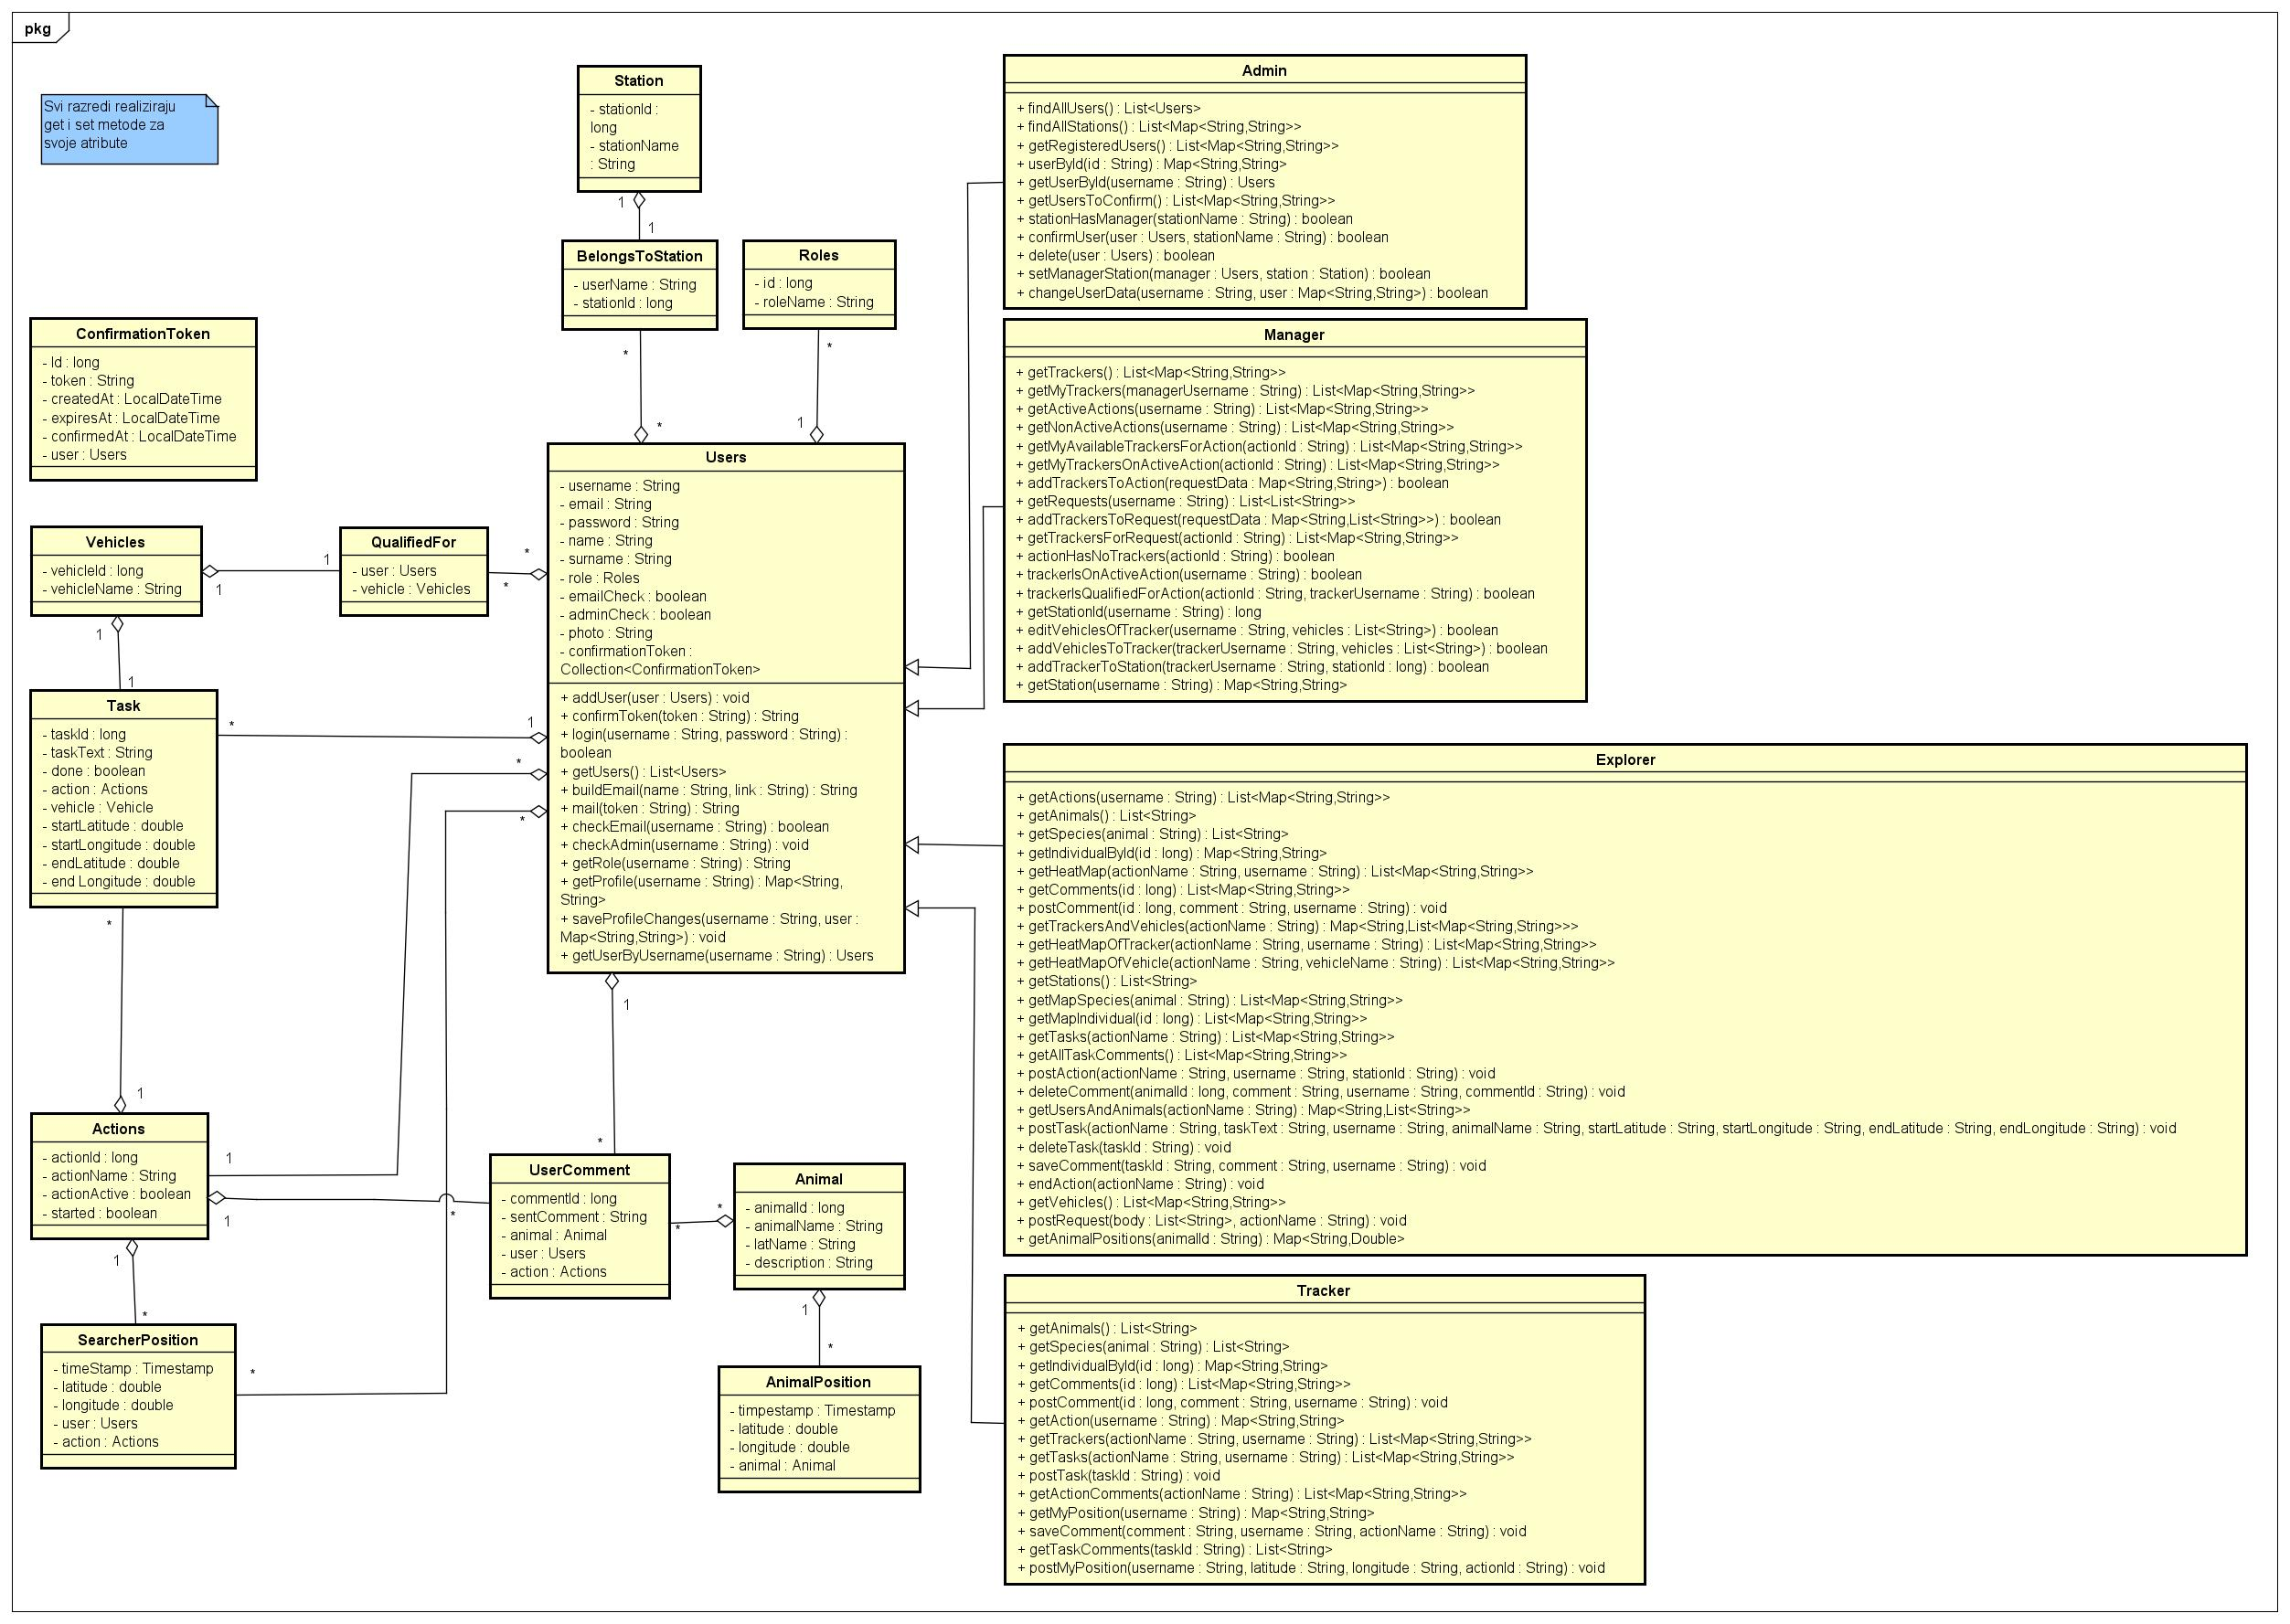
\includegraphics[scale=0.4]{slike/klasni_dijagram_models.jpg}
				\centering
				\caption{Dijagram razreda - dio Models}
				\label{fig:models}
			\end{figure}
			

			\textbf{\textit{dio 2. revizije}}\\			
			
			\textit{Prilikom druge predaje projekta dijagram razreda i opisi moraju odgovarati stvarnom stanju implementacije}
			
			
			
			\eject
		
		\section{Dijagram stanja}
			
			Dijagram stanja (slika \ref{fig:dijagram stanja - tragač}) opisuje dinamičko ponašanje sustava uslijed raznih mogućih
		događaja. Uspješnom prijavom prikazana je početna stranica korisnika u ulozi tragača. 
		Na početnoj stranici tragač bira jednu od tri opcije:
		\begin{packed_item}
		\item opciju \textit{Moj profil} dostupnu svakom korisniku, koja ga vodi na stranicu sa osobnim podacima, gdje ih može uređivati
		\item opciju \textit{O životinjama} koja ga vodi na stranicu na kojoj su prikazane sve vrste životinja u aplikaciji, a klikom na pojedinu vrstu dobiva popis jedinki te vrste i dalje klikom na pojedinu jedinku dobiva opširnije informacije specifično o toj jedinki
		\item opciju \textit{Moja akcija} koja ga vodi na stranicu s prikazom karte i dodatnim opcijama za pregled zadataka, ostalih tragača i praćenih životinja; nakon klika na praćene životinje ili ostale tragače, tragaču se prikazuje lista istih, a klikom na pojedinca te liste(tragača ili životinju) na karti mu se prikazuje trenutna pozicija odabranog
		\end{packed_item}

		\begin{figure}[H]
			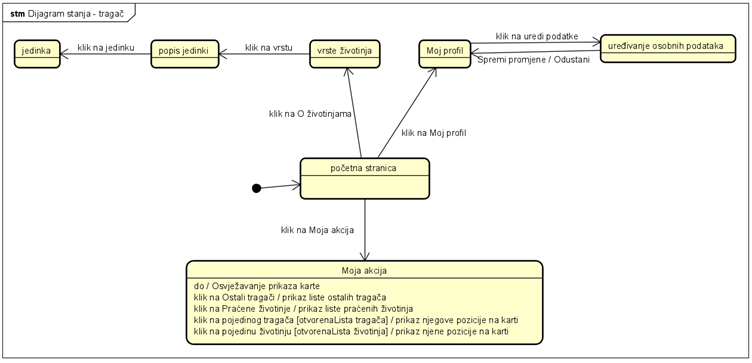
\includegraphics[scale=1]{slike/dijagram stanja - tragač.png}
			\centering
			\caption{Dijagram stanja - tragač}
			\label{fig:dijagram stanja - tragač}
		\end{figure}
			
			\eject 
		
		\section{Dijagram aktivnosti}

		Dijagramom aktivnosti na slici  \ref{fig:dijagram aktivnosti - stvaranje nove akcije} modelirano je stvaranje nove akcije korisnika u ulozi istraživača.
		Do postupka stvaranja nove akcije dolazi se sa stranice prikaza popisa akcija klikom na 
		\textit{Stvori novu akciju}. Na formularu za novu akciju se prilikom klika na \textit{Stvori novu akciju},
		prije spremanja podataka nove akcije u bazu, provjerava jesu li uneseni svi potrebni podatci i jesu li uneseni podatci ispravni.
		Nakon uspješnog stvaranja nove akcije, korisniku se prikazuje osvježen popis akcija, a ukoliko korisnik odustane od stvaranja nove akcije klikom na 
		\textit{Odustani} prikaz se vraća na popis akcija.

		\begin{figure}[H]
			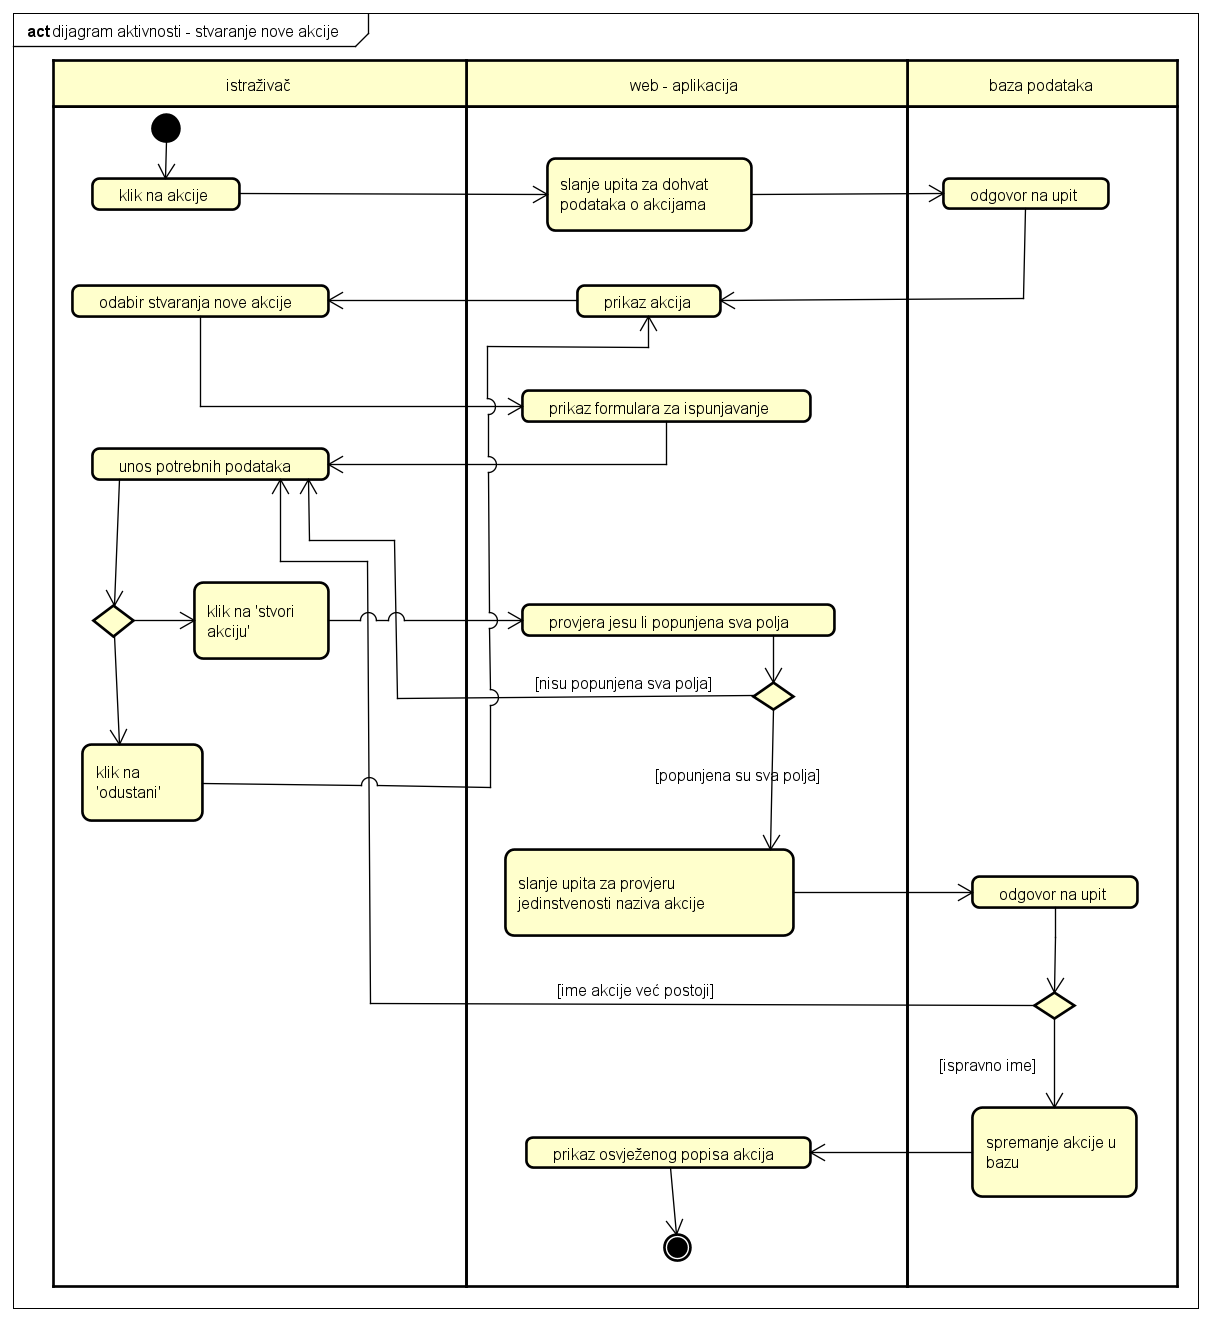
\includegraphics[scale=0.5]{slike/dijagram aktivnosti - stvaranje nove akcije.png}
			\centering
			\caption{Dijagram aktivnosti - stvaranje nove akcije}
			\label{fig:dijagram aktivnosti - stvaranje nove akcije}
		\end{figure}

			\eject


		\section{Dijagram komponenti}

		UML-dijagram komponenti je vrsta strukturnog UML-dijagrama koji
		prikazuje organizaciju i odnose komponenti koje čine programsku potporu. Pruža vizualni prikaz
		arhitekture sustava, naglašavajući modularnu strukturu i interakcije između komponenti, interne strukture i okoline.
		\newline Sustavu se pristupa preko dva razlicita sučelja. Preko sučelja za dohvat HTML, CSS i JS datoteka poslužuju se
datoteke koje pripadaju \textit{frontend} dijelu aplikacije. Router je komponenta koja na
upit s url određuje koja datoteka će se poslužiti na sučelje. Frontend dio se sastoji
od niza JavaScript datoteka koje su raspoređene u logičke cjeline nazvane po tipovima aktora koji im pristupaju. Sve JavaScript datoteke ovise o React biblioteci iz
koje dohvaćaju gotove komponente kao što su gumbi, forme i slično. Preko sučelja 
za dohvat JSON podataka pristupa se REST API komponenti. REST API poslužuje
podatke koji pripadaju \textit{backend} dijelu aplikacije. JpaRepository je sučelje Spring Data JPA projekta korišteno
za jednostavan dohvat i manipulaciju s podacima u bazi podataka, pružajući apstrakciju nad JPA 
(Java Persistence API) omogućavajući  izvođenje operacija nad entitetima bez potrebe za izravnim pisanjem SQL upita. Podaci koji su pristigli 
iz baze se šalju dalje MVC arhitekturi u obliku DTO  (Data transfer object). 
React-view komponenta preko dostupnih sučelja komunicira sa \textit{WildTrack} aplikacijom
te ovisno o korisnikovim akcijama osvježava prikaz i dohvaća nove podatke ili datoteke.
		
		\begin{figure}[H]
			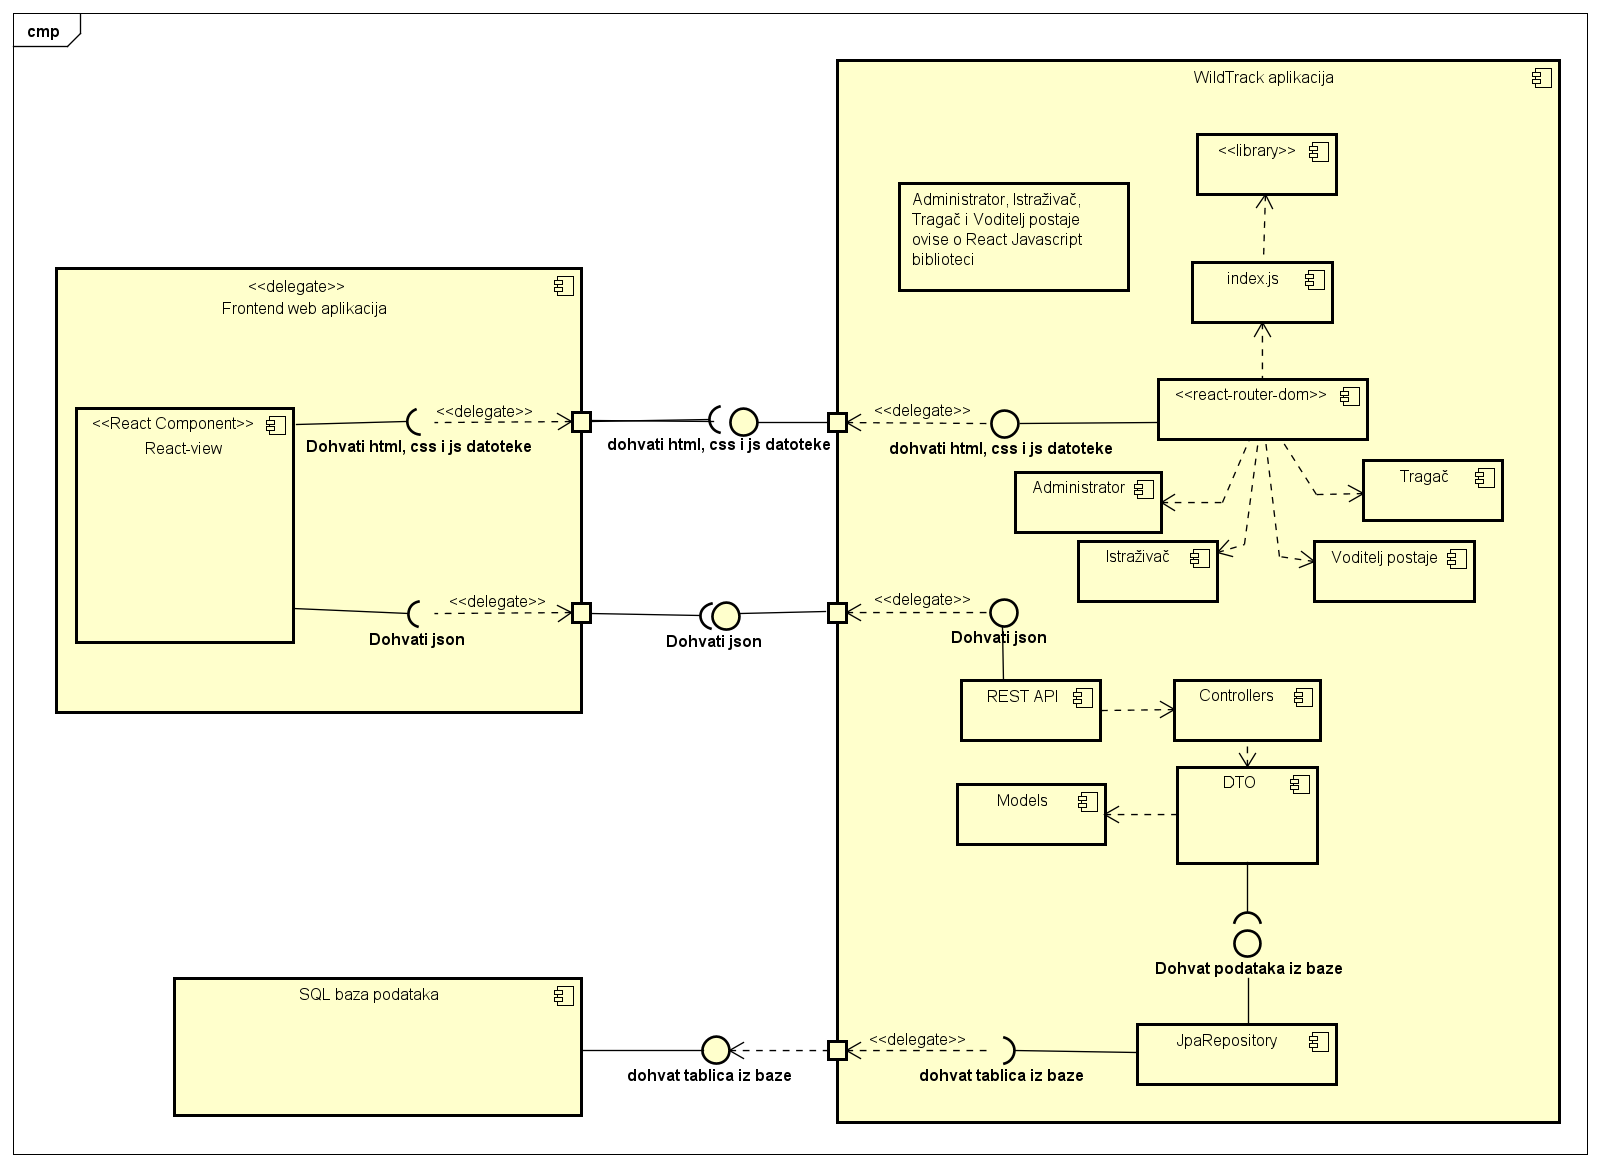
\includegraphics[scale=0.4]{slike/dijagram komponenti.png}
			\centering
			\caption{Dijagram komponenti}
			\label{fig:dijagram komponenti}
		\end{figure}
	\chapter{Implementacija i korisničko sučelje}
		
		
		\section{Korištene tehnologije i alati}
		
			
			  U izradi projekta većina digitalne komunikacije ostvarena je preko platforme
			  \textbf{WhatsApp} (\textit{https://web.whatsapp.com/} ).

			  Korištene su sljedeće tehnologije i alati:

			  \begin{packed_item}

				\item \textbf{Springboot}
					\begin{packed_item}
						\item open source radni okvir za kreaciju mikro-servisa, idealan za potrebe projekta
						\item u njemu je izrađen backend dio projekta 
						\item \textit{https://spring.io/projects/spring-boot}
					\end{packed_item}

				\item \textbf{React}
				\begin{packed_item}
					\item JavaScript biblioteka za izgradnju korisničkih sučelja 
					\item korišten za izradu čitavog frontenda dijela aplikacije s kojim korisnik dolazi u interakciju 
					\item provjerava ispravnost podataka unesenih u obrasce 
					\item \textit{ https://www.reactjs.org/}
				\end{packed_item}

				\item \textbf{PostgreSQL }
				\begin{packed_item}
					\item jezik u kojem je napravljena baza podataka  
					\item besplatan i open source sustav za upravljanje relacijskim bazama podataka s naglaskom na mogućnosti proširivanja  
					\item \textit{ https://www.postgresql.org/}
				\end{packed_item}
				
				\item \textbf{pgAdmin}
				\begin{packed_item}
					\item za upravljanje bazom podataka neovisno o backendu 
					\item \textit{ https://www.pgadmin.org/}
				\end{packed_item}

				\item \textbf{IntelliJ }
				\begin{packed_item}
					\item  IDE za javu u kojem je kodiran backend dio projekta 
					\item \textit{ https://www.jetbrains.com/idea/}
				\end{packed_item}

				\item \textbf{Visual Studio Code}
				\begin{packed_item}
					\item  uređivač izvornog koda za razne programske jezike
					\item  korišten za kodiranje frontend dijela projekta i projektne dokumentacije
					\item \textit{ https://code.visualstudio.com/}
				\end{packed_item}

				\item \textbf{Astah UML }
				\begin{packed_item}
					\item program za uređivanje svih vrsta UML dijagrama
					\item svi dijagrami u ovom dokumentu izrađeni su u Astahu 
					\item \textit{https://astah.net/products/astah-uml/}
				\end{packed_item}

				\item \textbf{GitHub }
				\begin{packed_item}
					\item  stranica za funkcionalno zajedničko stvaranje i uređivanje grupnog projekta 
					\item \textit{https://github.com/}
				\end{packed_item}

				\item \textbf{Latex}
				\begin{packed_item}
					\item programski jezik za pisanje strukturiranih tekstova, često korišten za stvaranje profesionalnih dokumenata
					\item koristi markup jezik koji prevodi u formatirane dokumente
					\item korišten za dokumentiranje projekta
					\item \textit{https://www.latex-project.org/}
				\end{packed_item}
				
				\item \textbf{Render}
				\begin{packed_item}
					\item cloud platforma za izradu i besplatno hostanje web-aplikacija i stranica
					\item korišten za puštanje \textit{backenda} i \textit{frontenda} u pogon i hostanje baze podataka
					\item \textit{https://www.render.com/}
				\end{packed_item}

				\item \textbf{Render}
				\begin{packed_item}
					\item cloud platforma za izradu i besplatno hostanje web-aplikacija i stranica
					\item korišten za puštanje \textit{backenda} i \textit{frontenda} u pogon i hostanje baze podataka
					\item \textit{https://www.render.com/}
				\end{packed_item}

				\item \textbf{Selenium}
				\begin{packed_item}
					\item program za automatizaciju web aplikacija u svrhe testiranja
					\item korišten za ispitivanje
					\item \textit{https://www.selenium.dev}
				\end{packed_item}
			\end{packed_item}
			

			 \eject 
		
	
		\section{Ispitivanje programskog rješenja}
			
			\subsection{Ispitivanje komponenti}
			Napravljen je java file za provođenje testova BackendApplicationTests.java sa JUnit testovima koji provjeravaju:

			\begin{packed_item}
					\item vraća li grešku funkcija za dohvaćanje korisnika s nepostojećim korisničkim imenom - testGetUserByUsernameThatDoesNotExist
					\item vraća li funkcija pravog korisnika za dohvaćanje korisnika s postojećim korisničkim imenom -  testGetUserByUsernameThatExists
					\item hoće li funkcija baciti grešku ako je uneseno ime nepostojeće postaje – testStationAlreadyHasManagerNonExistentStation
					\item hoće li funkcija za nepostojeći ID vozila baciti gresku – testFindVehicleByNonexistentId
					\item hoće li funkcija za dobro ime, ali lošu lozinku vratiti False – testLoginInvalidPassword
					\item hoće li funkcija vratiti True ako stanica već ima dodijeljenog voditelja - testStationAlreadyHasManager
				\end{packed_item}
			
			
			\begin{figure}[H]
				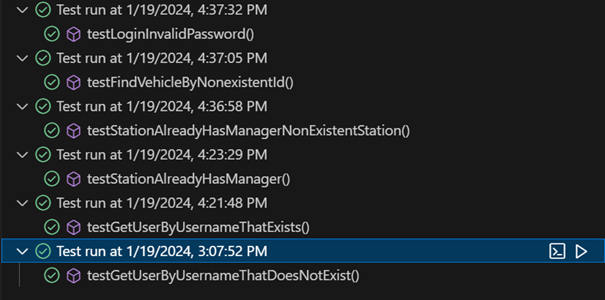
\includegraphics[scale=0.85]{slike/Zadovoljeni testovi.png}
				\centering
				\caption{Zadovoljeni testovi}
				\label{fig:Zadovoljeni testovi}
			\end{figure}

			\begin{figure}[H]
				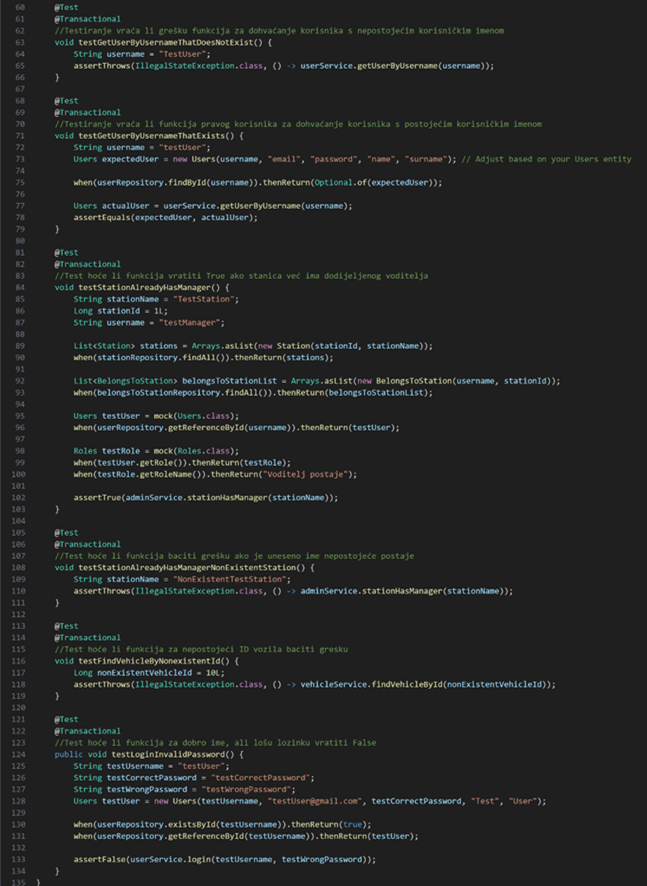
\includegraphics[scale=1]{slike/BackendApplicationTests.png}
				\centering
				\caption{Kod BackendApplicationTests.java}
				\label{fig:BackendApplicationTests}
			\end{figure}


			%%%%%%%%%%%%%%%%%%%%%%%%%%%%%%%%%%%%%%%%%%%%%%%%%%%%
			\subsection{Ispitivanje sustava}

			\textbf{Testovi sustava}
			Provedeni su testovi administratorove mogućnosti uređivanja podataka 
			korisnika, mogućnost voditelja postaje da na svoju postaju doda 
			tragače koji nisu dodijeljeni nijednoj drugoj postaji, mogućnost 
			istraživača da prouči informacije pojedinim jedinkama životinja 
			te mogućnost da mu se na karti prikazuju mjesta gdje se pojedine 
			vrste životinja kreću.
	
			\textit{\textbf{Mijenjanje podataka o korisnicima}}
			\newline
			Za test mijenjanja podataka o korisnicima koriste se ulazni podaci 
			„admin“ za korisničko ime te „password“ za lozinku. 

			

			Pritiskom na gumb „Prijava“ prikazuje nam se početna stranica za 
			administratora. Odaberemo opciju „Pregled korisnika“ te 
			na popisu korisnika odaberemo korisnika s korisničkim imenom 
			„tragac10“. Prikazuje nam se stranica sa svim podacima o navedenom 
			korisniku te opcije „Izbriši korisnika“ i „Promjeni podatke“. 
			Odaberemo opciju „Promijeni podatke“ te nakon što nam se otvori 
			forma za mijenjanje podataka, odaberemo polje ispod teksta „Email:“. 
			Kao novu adresu unesemo tragac15@gmail.hr te pritisnemo na tipku 
			„Spremi promjene“. Nakon toga ponovno nam se otvara stranica s 
			opcijama „Pregled korisnika“ i „Pregled zahtjeva“. Ponovno 
			odaberemo opciju „Pregled korisnika“ te pronađemo korisnika s 
			korisničkim imenom „tragač10“. Nakon što pritisnemo na tog korisnika,
			 otvara nam se stranica s njegovim podacima gdje možemo vidjeti 
			 njegovu izmijenjenu email adresu.

\begin{figure}[H]
				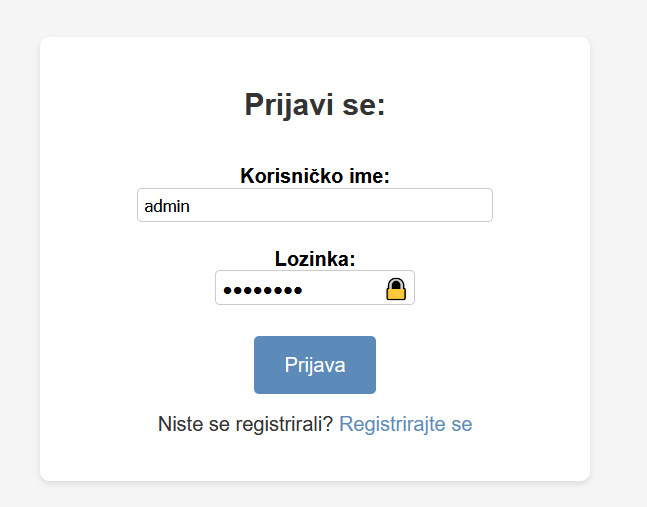
\includegraphics[scale=0.6]{slike/test11.png}
				\centering
				\caption{Mijenjanje podataka o korisnicima korak 1}
				\label{fig:Mijenjanje podataka o korisnicima korak 1}
			\end{figure}

			\begin{figure}[H]
				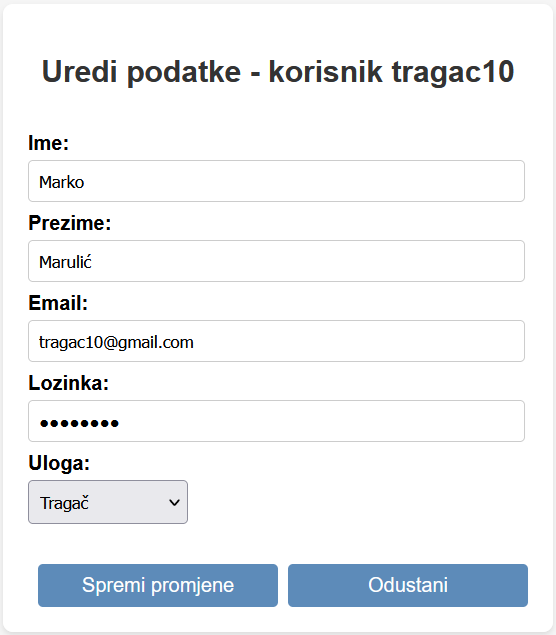
\includegraphics[scale=0.6]{slike/test12.png}
				\centering
				\caption{Mijenjanje podataka o korisnicima korak 2}
				\label{fig:Mijenjanje podataka o korisnicima korak 2}
			\end{figure}

			\begin{figure}[H]
				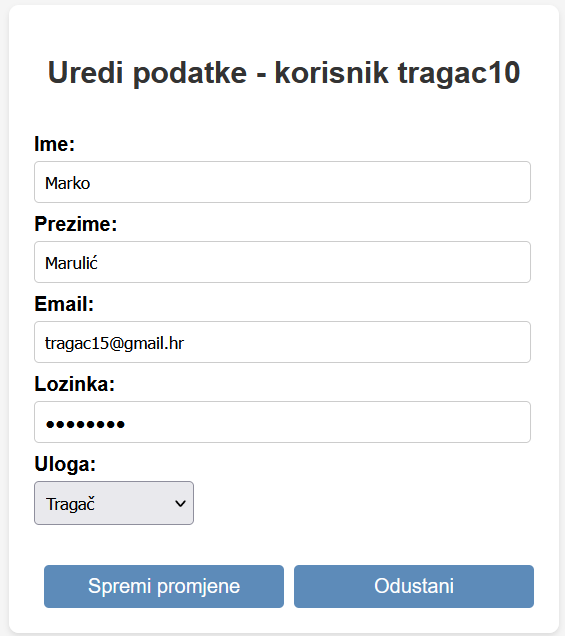
\includegraphics[scale=0.6]{slike/test13.png}
				\centering
				\caption{Mijenjanje podataka o korisnicima korak 3}
				\label{fig:Mijenjanje podataka o korisnicima korak 3}
			\end{figure}

			\begin{figure}[H]
				
\includegraphics[scale=0.7]{slike/test14.png}
				\centering
				\caption{Mijenjanje podataka o korisnicima korak 4}
				\label{fig:Mijenjanje podataka o korisnicima korak 4}
			\end{figure}



			\textit{\textbf{Dodavanje tragača na postaju}}
			\newline
			Za test dodavanja tragača na postaju u ulozi voditelja postaje koriste se ulazni 
			podaci „waiting“ za korisničko ime te „password“ za lozinku. Pritiskom na gumb 
			„Prijava“ prikazuje nam se početna stranica za korisnike u ulozi voditelja postaje. 
			Pojavljuje nam se tekst s postajom kojom upravlja prijavljeni voditelj te pet opcija 
			za odabir. Nude se opcije „Pregled svih tragača“, „Pregled svojih tragača“, „Pregled 
			akcija“, „Pregled zahtjeva“ te „Moj profil“ (u gornjem desnom kutu). Odaberemo opciju 
			„Pregled svih tragača“, nakon čega nam se otvara prozor s tekstom „Pregled svih tragača“ 
			te ispod njega popis svih tragača koji trenutno nemaju dodijeljenu postaju. 
			Pritiskom na kućicu ispod pripadajućeg tragača, nudi nam se šest različitih 
			vozila za dodjeljivanje kao sposobnosti odabranom tragaču. Odaberemo tragača s 
			imenom „test“ te prezimenom „tragac“. Nakon toga mu kao prijevozna sredstva dodijelimo 
			mogućnosti „pješke“ te „dronom“. Pritiskom na gumb „Potvrdi“ potvrđujemo svoj odabir. 
			Nakon što smo potvrdili svoj odabir, ponovno se otvara početna stranica korisnika u ulozi 
			voditelja postaje. Ovaj put odaberemo opciju „Pregled svojih tragača“, nakon čega nam se  
			otvara prozor sa tekstom „Lista svojih tragača“ te ispod njega popis svih tragača 
			dodijeljenih postaji, s njihovim osnovnim korisničkim podacima. Možemo vidjeti da se 
			sada i na popisu nalazi tragač s imenom „test“ i prezimenom „tragac“.



			\begin{figure}[H]
				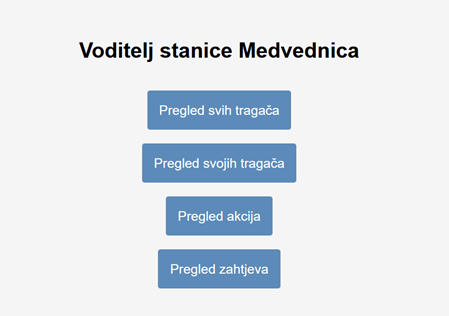
\includegraphics[scale=0.8]{slike/Dodavanje tragača na postaju korak 1.png}
				\centering
				\caption{Dodavanje tragača na postaju korak 1}
				\label{fig:Dodavanje tragača na postaju korak 1}
			\end{figure}

			\begin{figure}[H]
				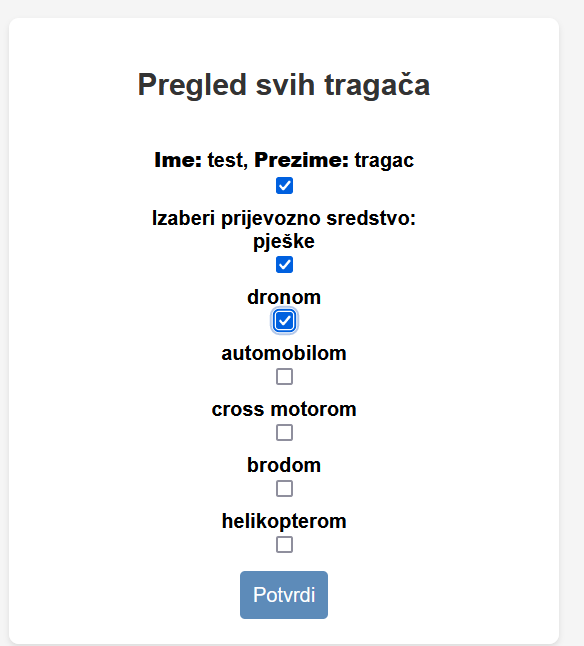
\includegraphics[scale=0.62]{slike/Dodavanje tragača na postaju korak 2.png}
				\centering
				\caption{Dodavanje tragača na postaju korak 2}
				\label{fig:Dodavanje tragača na postaju korak 2}
			\end{figure}

			\begin{figure}[H]
				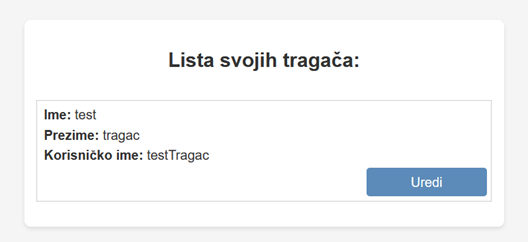
\includegraphics[scale=0.85]{slike/Dodavanje tragača na postaju korak 3.png}
				\centering
				\caption{Dodavanje tragača na postaju korak 3}
				\label{fig:Dodavanje tragača na postaju korak 3}
			\end{figure}


			\textit{\textbf{Pregled informacija o životinjama}}
			\newline

			Za test pregleda informacija o životinjama u ulozi istraživača koriste se ulazni 
			podaci „istrazivacXmouse“ za korisničko ime te „lozinka1“ za lozinku. Pritiskom 
			na gumb „Prijava“ prikazuje nam se početna stranica za korisnike u ulozi 
			istraživača. Za odabir nam se nude opcije „Popis akcija“, „Karta – životinje“,
			 „O životinjama“ te „Moj profil“ (u gornjem desnom kutu). Odaberemo opciju 
			 „O životinjama“. Otvara nam se izbornik s različitim vrstama životinja. 
			 Odaberemo opciju „Sivi vuk“ te nakon što nam se prikaže prozor s popisom 
			 jedinki te vrste, odaberemo opciju „Sivi vuk, id: 7“. Otvara nam se prozor u 
			 kojemu možemo vidjeti sliku pripadajuće vrste, njen latinski naziv, detaljan opis 
			 vrste te komentare ostalih korisnika vezanih uz navedenu jedinku. Dodatno, nudi 
			 nam se mogućnost brisanja te pisanja vlastitih komentara.



			\begin{figure}[H]
				\includegraphics[scale=0.6]{slike/Pregled informacija o životinjama korak 1.png}
				\centering
				\caption{Pregled informacija o životinjama korak 1}
				\label{fig:Pregled informacija o životinjama korak 1}
			\end{figure}

			\begin{figure}[H]
				\includegraphics[scale=0.55]{slike/Pregled informacija o životinjama korak 2.png}
				\centering
				\caption{Pregled informacija o životinjama korak 2}
				\label{fig:Pregled informacija o životinjama korak 2}
			\end{figure}

			\begin{figure}[H]
				\includegraphics[scale=0.6]{slike/Pregled informacija o životinjama korak 3.png}
				\centering
				\caption{Pregled informacija o životinjama korak 3}
				\label{fig:Pregled informacija o životinjama korak 3}
			\end{figure}


			\textit{\textbf{Pregled staništa vrste na karti}}
			\newline
			Za test pregleda staništa pojedine vrste životinja na karti u ulozi istraživača 
			koriste se ulazni podaci „ju54164“ za korisničko ime te „lozinka1“ za lozinku. 
			Pritiskom na gumb „Prijava“ prikazuje nam se početna stranica za korisnike u 
			ulozi istraživača. Za odabir nam se nude opcije „Popis akcija“, 
			„Karta – životinje“, „O životinjama“ te „Moj profil“ (u gornjem desnom kutu). 
			Odaberemo opciju „Karta – životinje“. Otvara nam se prozor u čijem se središtu 
			nalazi karta, a u gornjem lijevom kutu dvije opcije za prikaz na karti, 
			„Po vrsti“ te „Po jedinci“. Odaberemo opciju „Po vrsti“, nakon čega nam se 
			ispod pojavljuje popis svih mogućih vrsta. Pritiskom na gumb „Sivi sokol“, 
			na karti nam se pojavljuje heatmap svih povijesnih lokacija jedinki koje 
			pripadaju toj vrsti. 


			\begin{figure}[H]
				\includegraphics[scale=0.75]{slike/Pregled staništa vrste na karti korak 1.png}
				\centering
				\caption{Pregled staništa vrste na karti korak 1}
				\label{fig:Pregled staništa vrste na karti korak 1}
			\end{figure}

			\begin{figure}[H]
				\includegraphics[scale=1]{slike/Pregled staništa vrste na karti korak 2.png}
				\centering
				\caption{Pregled staništa vrste na karti korak 2}
				\label{fig:Pregled staništa vrste na karti korak 2}
			\end{figure}

			\begin{figure}[H]
				\includegraphics[scale=1]{slike/Pregled staništa vrste na karti korak 3.png}
				\centering
				\caption{Pregled staništa vrste na karti korak 3}
				\label{fig:Pregled staništa vrste na karti korak 3}
			\end{figure}




		%%%%%%%%%%%%%%%%%%%%%%%%%%%%%%%%%%%%%%%%%%%%%%%%%%%%%%%%%%%%%%%%%%%%%%%%%%%%%%%%%%%%%%%%%%%%%%%%%%%%%%%
		\section{Dijagram razmještaja}

		UML-dijagram razmještaja je vrsta strukturnog UML-dijagrama 
		koji prikazuje fizičku arhitekturu i konfiguraciju 
		razmještaja programskog sustava. Dijagram razmještaja koristan je 
		za vizualizaciju kako su komponente sustava raspoređene na fizičkim 
		računalima i kako međusobno komuniciraju.
		Na poslužiteljskom računalu se 
		nalaze web poslužitelj i poslužitelj baze podataka. Korisnici preko svog računala koriste web
		preglednik kako bi pristupili web aplikaciji. Sustav je baziran na arhitekturi 
		”klijent - poslužitelj”, a komunikacija između računala korisnika, 
		koji može biti tragač, istraživač, voditelj postaje ili administrator, i poslužitelja se 
		odvija preko HTTP veze, što je tipičan način komunikacije u web okolinama.

		\begin{figure}[H]
			\includegraphics[scale=0.7]{slike/dijagram razmještaja.png}
			\centering
			\caption{Dijagram razmještaja}
			\label{fig:dijagram razmještaja}
		\end{figure}
			\eject 
	%%%%%%%%%%%%%%%%%%%%%%%%%%%%%%%%%%%%%%%%%%%%%%%%%%%%%%%%%%%%%%%%%%%%%%%%%%%%%%%%%%%%%%%%%%%%%%%%%%%%%%%%%%%%%%%%%%%%%%%%%
	%%%%%%%%%%%%%%%%%%%%%%%%%%%%%%%%%%%%%%%%%%%%%%%%%%%%%%%%%%%%%%%%%%%%%%%%%%%%%%%%%%%%%%%%%%%%%%%%%%%%%%%%%%%%%%%%%%%%%%%%%
	%%%%%%%%%%%%%%%%%%%%%%%%%%%%%%%%%%%%%%%%%%%%%%%%%%%%%%%%%%%%%%%%%%%%%%%%%%%%%%%%%%%%%%%%%%%%%%%%%%%%%%%%%%%%%%%%%%%%%%%%%

		\section{Upute za puštanje u pogon}
		
			Puštanje web aplikacije u pogon sastoji se od tri segmenta:

			\begin{packed_item}
				\item Stvaranje baze podataka
				\item Puštanje \textit{backend-a} u pogon
				\item Puštanje \textit{frontend-a} u pogon
			\end{packed_item}

			\subsubsection{Stvaranje baze podataka}

			Baza podataka besplatno je spremljena na web-oblaku render.com. 
			Ona se postavlja i osposobljava sljedećim koracima:

			\begin{packed_enum}
				\item Stvaranje nove baze
				
				\begin{packed_item}
					\item Potrebno je (nakon registracije na render.com) odabrati opciju New te na padajućem izborniku PostgreSQL
					\item Pojavljuje se izbornik koji ispunjavamo kao na slici \ref{fig:postavljanje baze1}
					\item Biramo \textit{Create Database}
				\end{packed_item}

			\begin{figure}[H]
				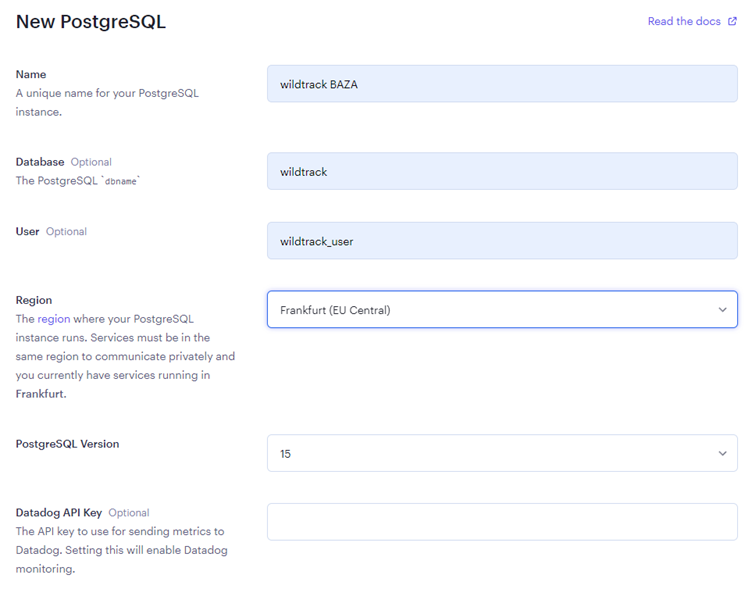
\includegraphics[scale=1]{slike/postavljanje baze1.png}
				\centering
				\caption{Stvaranje nove PostgreSQL baze}
				\label{fig:postavljanje baze1}
			\end{figure}

			 \item Dohvat podataka za spajanje
			 \begin{packed_item}
				\item Odabiremo \textit{Dashboard -  wildtrack BAZA -  Info}
				\item Spuštamo stranicu do izbora \textit{Connections} sa informacijama potrebnim za spajanje na bazu (slika \ref{fig:postavljanje baze2}).
			\end{packed_item}

			\begin{figure}[H]
				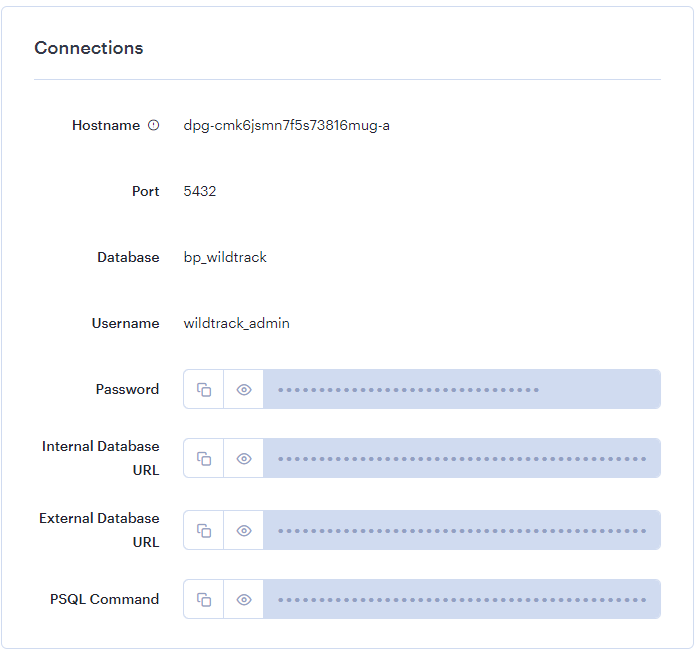
\includegraphics[scale=1]{slike/postavljanje baze2.png}
				\centering
				\caption{Dohvat podataka za spajanje baze}
				\label{fig:postavljanje baze2}
			\end{figure}

			\item Spajanje putem pgAdmina
			\begin{packed_item}
				\item Odabiremo \textit{Object - Create - Server}
				\item Na kartici \textit{General} unosimo ime servera kojeg otvaramo u pgAdminu
				\item Na kartici \textit{Connection} unosimo podatke kao na slici \ref{fig:postavljanje baze3} i spremamo ih sa \textit{Save}
			\end{packed_item}

			\begin{figure}[H]
				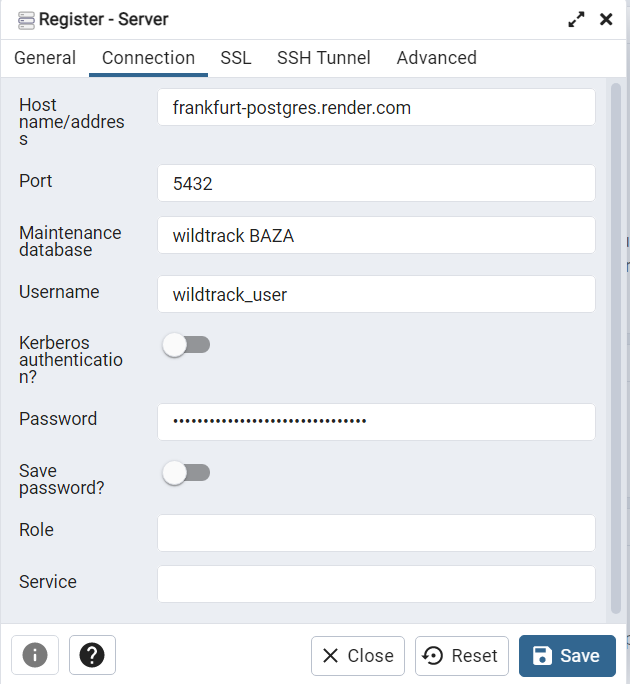
\includegraphics[scale=1]{slike/postavljanje baze3.png}
				\centering
				\caption{Unos podataka za spajanje baze}
				\label{fig:postavljanje baze3}
			\end{figure}

			\item Spajanje iz \textit{backenda}
			\begin{packed_item}
				\item U \textit{src/main/resources/application.properties} upisujemo naredbe sa slike \ref{fig:postavljanje baze4}
			\end{packed_item}
			
			\begin{figure}[H]
				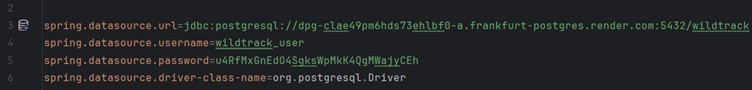
\includegraphics[scale=1]{slike/postavljanje baze4.png}
				\centering
				\caption{Spajanje baze iz \textit{backenda}}
				\label{fig:postavljanje baze4}
			\end{figure}


			\end{packed_enum}

			\subsubsection{Puštanje backenda u pogon}

			Backend dio projekta također koristi render.com za puštanje u pogon. Preduvjeti za to su:
			\begin{packed_item}
				\item Dodavanje Dockerfile-a prikazanog na slici \ref{fig:dockerfile}
				\item povezivanje s GitHub-om na renderu
			\end{packed_item}

			\begin{figure}[H]
				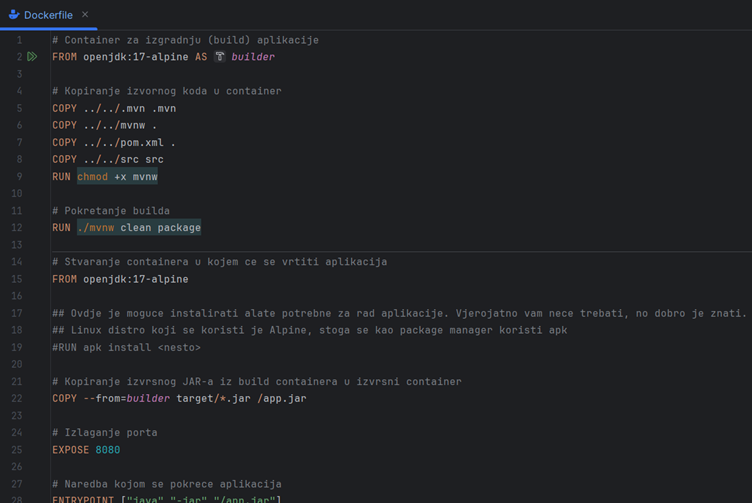
\includegraphics[scale=1]{slike/dockerfile.png}
				\centering
				\caption{Potrebni Dockerfile}
				\label{fig:dockerfile}
			\end{figure}

			Stvaranje backenda postižemo na sljedeći način:
			\begin{packed_item}
				\item Odabiremo na renderu \textit{New - Web Service}
				\item Odabiremo željeni GitHub repozitorij
				\item Unosimo tražene podatke i potvrđujemo s \textit{Create Web Service}
			\end{packed_item}

			\subsubsection{Puštanje frontenda u pogon}

			Frontend dio projekta također koristi render.com za puštanje u pogon. Preduvjeti za to su:
			
			\begin{packed_item}
				\item U IzvorniKod/package.json dodajemo dependency-e (primarno http-proxy-middleware, dotenv, express) kao na slici \ref{fig:frontendDeploy1}
				
			\begin{figure}[H]
				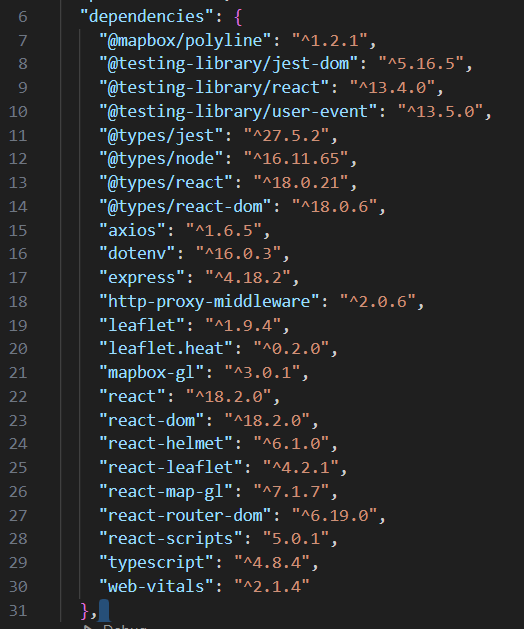
\includegraphics[scale=1]{slike/frontendDeploy1.png}
				\centering
				\caption{Dio koda package.json \textit{dependency}}
				\label{fig:frontendDeploy1}
			\end{figure}
			
				\item U IzvorniKod/package.json dodajemo kod kao na slici \ref{fig:frontendDeploy2} zbog funkcionalnosti Node-a
				
			\begin{figure}[H]
				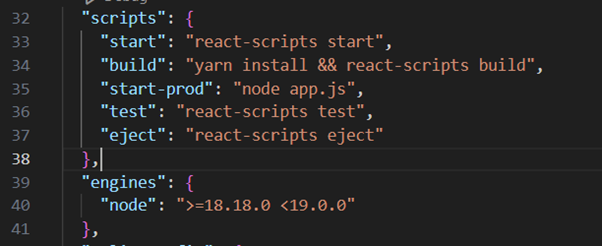
\includegraphics[scale=1]{slike/frontendDeploy2.png}
				\centering
				\caption{Dio koda package.json za funkcionalnost\textit{Node-a}}
				\label{fig:frontendDeploy2}
			\end{figure}
			
				\item Dodajemo /src/setupProxy.js koji služi kao proxy server za lokalni development (preusmjerava api pozive na localhost:8080)
				\item Dodajemo app.js, u kojem se nalazi express server za produkcijski proxy i posluživanje \textit{frontenda} (slika \ref{fig:frontendDeploy3})
			
			\begin{figure}[H]
				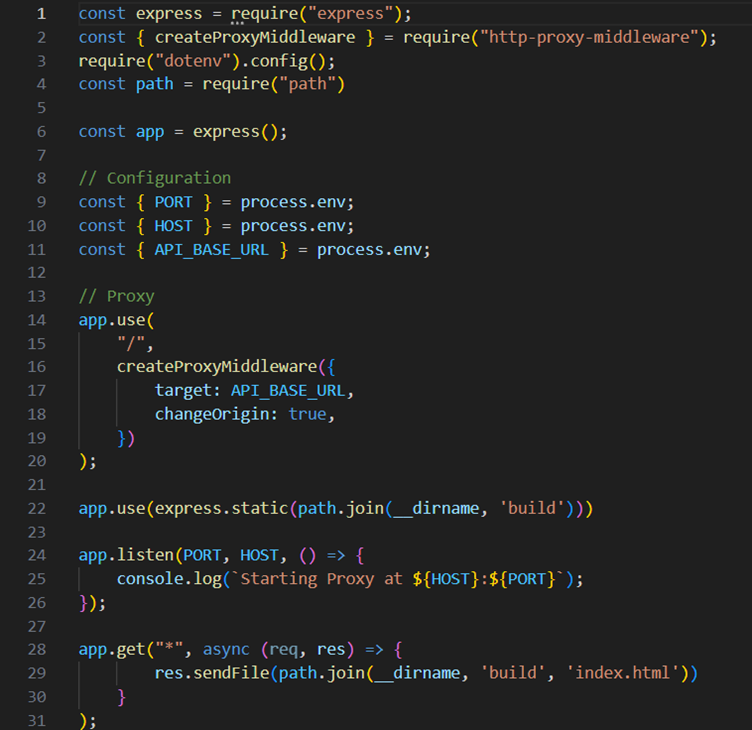
\includegraphics[scale=1]{slike/frontendDeploy3.png}
				\centering
				\caption{Kod datoteke app.js}
				\label{fig:frontendDeploy3}
			\end{figure}

			Stvaranje frontenda postižemo na sljedeći način:
			\begin{packed_item}
				\item Odabiremo na renderu \textit{New - Web Service}
				\item Odabiremo željeni GitHub repozitorij
				\item Unosimo tražene podatke (slika \ref{fig:frontendDeploy4})
				\item Potvrđujemo s \textit{Create Web Service}
			\end{packed_item}

			\begin{figure}[H]
				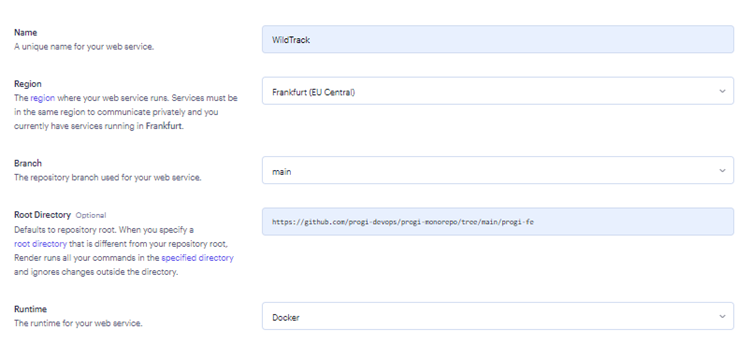
\includegraphics[scale=1]{slike/frontendDeploy4.png}
				\centering
				\caption{Spajanje \textit{frontenda}}
				\label{fig:frontendDeploy4}
			\end{figure}

		
		\end{packed_item}
			
			

			

			



			\eject 
	\chapter{Zaključak i budući rad}
		
Zadatak naše grupe Aristos bio je razvoj web aplikacije koja olakšava koordinaciju prilikom 
praćenja divljih životinja. Rad na projektu sadržavao je mnoge očekivane i neočekivane izazove 
i zapreke koje smo rješavali kroz marljivu suradnju.
\newline Nakon dodjele projektnog zadatka, oformili smo podjedinice za razvoj \textit{frontend-a}, razvoj 
\textit{backend-a} i pisanje dokumentacije te počeli s raspodjelom rada na incijalnim koracima projekta.
 Organizacija vremena i rada te podjela poslova bili su od ključne važnosti u napretku projekta, 
 baš kao i međusobna suradnja. 
 Kao zajednički oslonac koristili smo rukom crtanu skicu koja prikazuje idejni izgled početne stranice 
 i njezino grananje na razne funkcionalnosti za različite uloge korisnika. Članovi su se, zbog 
 nedostatka iskustva u razvoju implementacijskih rješenja, morali angažirati u samostalnom učenju 
 odabranih alata i programskih jezika kako bi postigli postavljene ciljeve i rokove. 
\newline Naša \textit{WildTrack} web aplikacija ima još prostora za potencijalna buduća unapređenja 
koja smo mogli ostvariti uz malo više vremena i vještine, poglavito stvaranje mobilne aplikacije 
da se približi suvremenim korisnicima. 
\newline Unatoč prostoru za usavršavanje na određenim aspektima aplikacije, 
koji je posljedica neiskustva, kao tim smo zadovoljni postignutim konačnim rezultatom, 
vremenom uloženim u projekt te znanjem koje smo stekli radeći ga. 
Zajedničko stvaranje web-aplikacije koristilo je kao vrijedno novo iskustvo svakom od članova i približilo nas 
		\eject 
	\chapter*{Popis literature}
		\addcontentsline{toc}{chapter}{Popis literature}		
		
		\begin{enumerate}
			
			
			\item  Programsko inženjerstvo, FER ZEMRIS, \url{http://www.fer.hr/predmet/proinz}
			
			\item  W3Schools, \url{https://www.w3schools.com/}
			
			\item Latex Forum, \url{https://latex.org/forum/index.php}
			
			\item Spring Boot, \url{https://spring.io/projects/spring-boot}
			
			\item  I. Sommerville, "Software engineering", 8th ed, Addison Wesley, 2007.
			
			\item  T.C.Lethbridge, R.Langaniere, "Object-Oriented Software Engineering", 2nd ed. McGraw-Hill, 2005.
			
			\item  I. Marsic, Software engineering book``, Department of Electrical and Computer Engineering, Rutgers University, \url{http://www.ece.rutgers.edu/~marsic/books/SE}
			
			\item  The Unified Modeling Language, \url{https://www.uml-diagrams.org/}
			
			\item  Astah Community, \url{http://astah.net/editions/uml-new}
			
			\item  \url{https://play.google.com/store/apps/details?id=com.mpio.movebank&hl=en&gl=US}
			
			\item  \url{https://play.google.com/store/apps/details?id=com.tips.dikihzhivotnyh&hl=hr}
		\end{enumerate}
		
		 
	
	
	\begingroup
	\renewcommand*\listfigurename{Indeks slika i dijagrama}
	%\renewcommand*\listtablename{Indeks tablica}
	%\let\clearpage\relax
	\listoffigures
	%\vspace{10mm}
	%\listoftables
	\endgroup
	\addcontentsline{toc}{chapter}{Indeks slika i dijagrama}


	
	\eject 
		
	\chapter*{Dodatak: Prikaz aktivnosti grupe}
		\addcontentsline{toc}{chapter}{Dodatak: Prikaz aktivnosti grupe}
		
		\section*{Dnevnik sastajanja}
						
		\begin{packed_enum}
			\item  sastanak
			
			\item[] \begin{packed_item}
				\item Datum: 20.listopada 2023.
				\item Prisustvovali: F. Vuković, M. Pongrac, M. Kukolj, S. Troskot, J. Udovičić, D. Jurič
				\item Teme sastanka:
				\begin{packed_item}
					\item  sastanak sa asistentom
					\item analiza zadatka
				\end{packed_item}
			\end{packed_item}

			\item  sastanak
			
			\item[] \begin{packed_item}
				\item Datum: 25.listopada 2023.
				\item Prisustvovali: F. Vuković, M. Pongrac, M. Kukolj, S. Troskot, J. Udovičić, D. Jurič
				\item Teme sastanka:
				\begin{packed_item}
					\item  određivanje izgleda aplikacije
					\item definiranje funkcionalnih zahtjeva
					\item raspodjela poslova 
				\end{packed_item}
			\end{packed_item}
			
			\item  sastanak
			\item[] \begin{packed_item}
				\item Datum: 4.studenoga 2023.
				\item Prisustvovali: F. Vuković, M. Pongrac, M. Kukolj, S. Troskot, J. Udovičić, D. Jurič, G. Mihaljević
				\item Teme sastanka:
				\begin{packed_item}
					\item  pregled i popravak dijagrama   
					\item  dogovor u kojem jeziku i programima programiramo 
					\item raspodjela poslova 
				\end{packed_item}
			\end{packed_item}

			\item  sastanak
			\item[] \begin{packed_item}
				\item Datum: 10.studenoga 2023.
				\item Prisustvovali: F. Vuković, M. Pongrac, M. Kukolj, S. Troskot, J. Udovičić, D. Jurič
				\item Teme sastanka:
				\begin{packed_item}
					\item  sastanak sa demonstratorom - pregled dosadašnjeg rada
					\item  osmišljavanje stranice i pojedinih pregleda
					\item raspodjela poslova 
				\end{packed_item}
			\end{packed_item}

			\item  sastanak
			\item[] \begin{packed_item}
				\item Datum: 16.studenoga 2023.
				\item Prisustvovali: F. Vuković, M. Pongrac, M. Kukolj, S. Troskot, J. Udovičić, D. Jurič, G. Mihaljević
				\item Teme sastanka:
				\begin{packed_item}
					\item  provjera svega napravljenoga
					\item dogovor tko će koji dio prepraviti 
					\item dogovor što trebamo dodati
				\end{packed_item}
			\end{packed_item}

			\item  sastanak
			\item[] \begin{packed_item}
				\item Datum: 14.prosinca 2023.
				\item Prisustvovali: F. Vuković, M. Pongrac, M. Kukolj, S. Troskot, J. Udovičić, D. Jurič, G. Mihaljević
				\item Teme sastanka:
				\begin{packed_item}
					\item dogovor oko izgleda stranice
					\item dogovor oko izgleda baze podataka
					\item raspodjela poslova
				\end{packed_item}
			\end{packed_item}

			\item  sastanak
			\item[] \begin{packed_item}
				\item Datum: 15.prosinca 2023.
				\item Prisustvovali: F. Vuković, M. Pongrac, M. Kukolj, S. Troskot, J. Udovičić, D. Jurič
				\item Teme sastanka:
				\begin{packed_item}
					\item dogovor sa asistentom i demonstratorom
					\item raspodjela poslova
					\item detaljan dogovor oko izgleda stranice voditelja i istraživača
				\end{packed_item}
			\end{packed_item}

			\item  sastanak
			\item[] \begin{packed_item}
				\item Datum: 09.siječnja 2024.
				\item Prisustvovali: F. Vuković, M. Pongrac, M. Kukolj, S. Troskot, J. Udovičić, D. Jurič
				\item Teme sastanka:
				\begin{packed_item}
					\item provjera napravljenog
					\item dogovor izgleda stranice za tragača
					\item raspodjela poslova
				\end{packed_item}
			\end{packed_item}


			\item  sastanak
			\item[] \begin{packed_item}
				\item Datum: 15.siječnja 2023.
				\item Prisustvovali: F. Vuković, M. Pongrac, M. Kukolj, S. Troskot, J. Udovičić, D. Jurič
				\item Teme sastanka:
				\begin{packed_item}
					\item provjera napravljenog
					\item dogovor oko dodavanja posljednjih funcionalnsti
				\end{packed_item}
			\end{packed_item}
			%
			
		\end{packed_enum}
		
		\eject
		\section*{Tablica aktivnosti}
		
			\begin{longtblr}[
					label=none,
				]{
					vlines,hlines,
					width = \textwidth,
					colspec={X[7, l]X[1, c]X[1, c]X[1, c]X[1, c]X[1, c]X[1, c]X[1, c]}, 
					vline{1} = {1}{text=\clap{}},
					hline{1} = {1}{text=\clap{}},
					rowhead = 1,
				} 
			
				\SetCell[c=1]{c}{} & \SetCell[c=1]{c}{\rotatebox{90}{\textbf{Josipa Udovičić}}} & \SetCell[c=1]{c}{\rotatebox{90}{\textbf{Franjo Vuković}}} &	\SetCell[c=1]{c}{\rotatebox{90}{\textbf{Stela Troskot}}} & \SetCell[c=1]{c}{\rotatebox{90}{\textbf{Marko Pongrac}}} &	\SetCell[c=1]{c}{\rotatebox{90}{\textbf{Marko Kukolj}}} & \SetCell[c=1]{c}{\rotatebox{90}{\textbf{Domagoj Jurič}}} &	\SetCell[c=1]{c}{\rotatebox{90}{\textbf{Gregor Mihaljević}}} \\  
				Upravljanje projektom 		& 5 & 3 & 1 &  &  &  & \\ 
				Opis projektnog zadatka 	& 4 &  &  &  &  &  & \\ 
				
				Funkcionalni zahtjevi       & 1 &  &  &  &  &  &  \\ 
				Opis pojedinih obrazaca 	&  &  & 2 &  &  & 2 &  \\ 
				Dijagram obrazaca 			&  & 3 &  & 3 & 3 &  &  \\ 
				Sekvencijski dijagrami		&  & 2 &  & 2 & 2 &  &  \\ 
				Opis sekvencijskih dijagrama	&  &  &  & & 2 &  &  \\ 
				Opis ostalih zahtjeva 		&  &  & 11 &  &  & 11 &  \\ 

				Arhitektura i dizajn sustava	 & 3 &  &  &  &  &  &  \\ 
				Baza podataka(opis)				& 1 &  &  &  &  &  & 3  \\ 
				Dijagram razreda 			&  & 6 &  & 6 & 9 &  &   \\ 
				Dijagram stanja				&  &  & 3 &  &  &  &  \\ 
				Dijagram aktivnosti 		&  &  & 3 &  &  &  &  \\ 
				Dijagram komponenti			&  &  & 4 &  &  &  &  \\ 
				Korištene tehnologije i alati 		&  &  & 1 &  &  &  &  \\ 
				Ispitivanje programskog rješenja 	&  &  &  & 9 &  &  &  \\ 
				Dijagram razmještaja			&  &  & 2 &  &  &  &  \\ 
				Upute za puštanje u pogon 		& 2 & 8 &  &  & 3 &  &  \\  
				Dnevnik sastajanja 			& 1 &  &  &  &  &  &  \\ 
				Zaključak i budući rad 		&  &  & 1 &  &  &  &  \\  
				Popis literature 			& 1 &  &  &  &  &  &  \\  
				&  &  &  &  &  &  &  \\ \hline 
				izrada početne stranice(registracija) 	& 7 &  &  &  &  &  &  \\  
				izrada baze podataka	 	&  & 4 &  & 4 &  &  & \\  
				spajanje s bazom podataka	&  & 2 &  & 2 & 5 &  &  \\ 
				back end					&  & 350 &  & 260 & 180 &  &  \\  
				front end					& 300 &  & 20 &  &  & 200 &\\ 
			\end{longtblr}
					
					
		\eject
		\section*{Dijagrami pregleda promjena}
		
		\textbf{\textit{dio 2. revizije}}\\
		
		\textit{Prenijeti dijagram pregleda promjena nad datotekama projekta. Potrebno je na kraju projekta generirane grafove s gitlaba prenijeti u ovo poglavlje dokumentacije. Dijagrami za vlastiti projekt se mogu preuzeti s gitlab.com stranice, u izborniku Repository, pritiskom na stavku Contributors.}
		
	


\end{document} %naredbe i tekst nakon ove naredbe ne ulaze u izgrađen dokument 


